\documentclass[12pt]{article}

\usepackage[utf8]{inputenc}
%\usepackage[T1]{fontenc}

\usepackage{geometry}
\geometry{a4paper}
\usepackage{graphicx}
\usepackage{float}
\usepackage[italian]{babel}
\usepackage{listings}
\usepackage{xcolor}
\usepackage{url}
\usepackage{hyperref}

\definecolor{codegreen}{rgb}{0,0.6,0}
\definecolor{codegray}{rgb}{0.5,0.5,0.5}
\definecolor{codepurple}{rgb}{0.58,0,0.82}
\definecolor{backcolour}{rgb}{0.95,0.95,0.92}

\lstdefinestyle{mystyle}{
    backgroundcolor=\color{backcolour},   
    commentstyle=\color{codegreen},
    keywordstyle=\color{magenta},
    numberstyle=\tiny\color{codegray},
    stringstyle=\color{codepurple},
    basicstyle=\ttfamily\footnotesize,
    breakatwhitespace=false,         
    breaklines=true,                 
    captionpos=b,                    
    keepspaces=true,                 
    numbers=left,                    
    numbersep=5pt,                  
    showspaces=false,                
    showstringspaces=false,
    showtabs=false,                  
    tabsize=2
}

\lstset{style=mystyle}

\linespread{1.2}
\setlength{\parindent}{0pt}

\begin{document}

\renewcommand{\labelenumii}{\arabic{enumi}.\arabic{enumii}}
\renewcommand{\labelenumiii}{\arabic{enumi}.\arabic{enumii}.\arabic{enumiii}}
\renewcommand{\labelenumiv}{\arabic{enumi}.\arabic{enumii}.\arabic{enumiii}.\arabic{enumiv}}
%----------------------------------------------------------------------------------------
%	TITOLO
%----------------------------------------------------------------------------------------

\begin{titlepage}

    \newcommand{\HRule}{\rule{\linewidth}{0.5mm}}

    \center

    \textsc{\Large Relazione di progetto di "Smart City e Tecnologie Mobili"}\\[0.5cm]

    \HRule \\[0.4cm]
    { \huge \bfseries CityTwin}\\[0.4cm]
    \HRule \\[1.5cm]

    \vfill

    \begin{flushleft}
        \emph{Numero del gruppo: 128}\\[1cm]
        \emph{Componenti del gruppo: Eddie Barzi, Filippo Vissani}\\[3cm]
    \end{flushleft}

\end{titlepage}

%----------------------------------------------------------------------------------------
%	INDICE
%----------------------------------------------------------------------------------------

\tableofcontents

\newpage

%----------------------------------------------------------------------------------------
%	INTRODUZIONE
%----------------------------------------------------------------------------------------

\section{Introduzione}

Il progetto CityTwin si propone di realizzare la simulazione di un sistema di digital twin nel contesto della smart city. In particolare, si vuole realizzare un sistema che sia in grado di catturare e rappresentare in formato digitale il comportamento delle varie entità presenti all'interno della città. Questo può portare ad una serie di benefici, alcuni dei quali vengono elencati di seguito:

\begin{itemize}
    \item Rilevazione di possibili problematiche e intervento tempestivo/automatizzato.
    \item Riduzione del consumo energetico.
    \item Rilevazione della qualità dell'aria e dell'acqua.
    \item Analisi dell'inquinamento acustico.
    \item Ottimizzazione della mobilità urbana.
\end{itemize}

La simulazione sarà composta da due tipologie di nodi: i nodi Mainstay, che rappresentano la struttura portante del sistema, e i nodi Resource, che rappresentano astrazioni di sensori, attuatori o entità più complesse.

I nodi Mainstay si occupano di scambiare informazioni con i nodi Resource, rilevare eventuali malfunzionamenti e salvare in modo persistente le informazioni rilevate dai nodi Resource. I nodi Mainstay devono essere sempre sincronizzati tra loro, in modo da poter garantire la coerenza dei dati.

I nodi Resource, invece, si occupano di rilevare informazioni e comunicarle ai nodi Mainstay nel caso in cui vengono considerati come sensori. Nel caso in cui i nodi Resource rappresentino attuatori, invece, si occupano di ricevere informazioni dai nodi Mainstay e agire di conseguenza.

Per la memorizzazione delle dello stato dei nodi viene disposto un servizio apposito di persistenza dei dati. Tale servizio viene utilizzato sia dai nodi Mainstay che da altri clienti, come ad esempio il pannello di controllo.

L'utente potrà visualizzare lo stato attuale del sistema, lo storico dei dati ed eventuali statistiche, nonché interagire con il sistema tramite GUI, ad esempio per intervenire dopo la rilevazione di un incendio.

Per la realizzazione del progetto verranno utilizzate le seguenti tecnologie:

Akka\cite{akka} è un toolkit open source e runtime che semplifica la costruzione di applicazioni concorrenti e distribuite sulla JVM. Questo toolkit supporta diversi modelli di programmazione per la concorrenza, ma enfatizza la concorrenza basata su attori.

I componenti principali del progetto, quali Mainstay e Resource, verranno modellati sulla base del paradigma ad attori e verranno realizzati utilizzando Akka in combinazione con il linguaggio Scala 3\cite{scala}.

Per quanto riguarda il servizio di persistenza dei dati, utile per visualizzare le statistiche, verrà utilizzato MongoDB\cite{mongodb}, un database non relazionale orientato ai documenti. Questo database verrà utilizzato per salvare in modo persistente i dati rilevati dai nodi Mainstay.
Il servizio di persistenza verrà realizzato come modulo separato, per questo motivo si sceglie di implementare un layer scritto in JavaScript, che esponga delle API utilizzabili sia dai nodi Mainstay che da altri clienti.

Sulla base dei linguaggi scelti, verranno adottati Simple Build Tool (SBT)\cite{sbt} per Scala 3 e Node Package Manager (NPM)\cite{npm} per JavaScript per la gestione delle dipendenze e la compilazione del codice.

Per semplificare l'avvio del sistema distribuito e garantire la scalabilità verrà utilizzato Docker\cite{docker}, un progetto open source che automatizza il deployment di applicazioni all'interno di contenitori software.

\newpage

%----------------------------------------------------------------------------------------
%	STATO DELL'ARTE
%----------------------------------------------------------------------------------------

\section{Stato dell'arte}

La piattaforma open source di riferimento per la realizzazione di sistemi di smart city è Snap4City\cite{Snap4City}, sviluppata da DISIT Lab dell'Università di Firenze\cite{DISIT}. Questa piattaforma offre una vasta gamma di funzionalità per la raccolta, l'elaborazione e la visualizzazione dei dati urbani, consentendo decisioni informate in tempo reale. Snap4City permette anche l'integrazione di dati provenienti da fonti esterne, come dati geospaziali, informazioni meteorologiche o flussi di traffico, per creare nuovi servizi.

\subsection{Snap4City}

Snap4City offre le seguenti funzionalità chiave:

\begin{itemize}
    \item Acquisizione dati da sorgenti diverse, inclusi OpenData, GIS territoriali, dispositivi IoT, sensori industriali e social media, con vari protocolli di comunicazione.
    \item Aggregazione dati con il modello semantico unificato Km4City, permettendo di riconciliare dati complessi.
    \item Data analytics in tempo reale per produrre risultati diretti e inferiti, utilizzando strumenti di machine learning e calcolo massivo.
    \item Visualizzazione dei dati tramite dashboard interattive, mobile e altri dispositivi.
    \item Creazione di sinottici e dashboard personalizzate connesse a soluzioni DCS (Dynamic Control System).
\end{itemize}

\subsection{Confronto tra Snap4City e il Progetto CityTwin}
Pur affrontando obiettivi simili di monitoraggio e gestione delle smart city, Snap4City e il progetto CityTwin presentano alcune differenze.

\subsubsection{Architettura e Scopo}
Snap4City è una piattaforma completa che si basa sulla raccolta di dati reali provenienti da varie fonti, consentendo un monitoraggio accurato dell'ambiente urbano. La piattaforma offre strumenti per la visualizzazione dei dati e l'analisi, consentendo agli utenti di ottenere insights significativi sull'ambiente urbano effettivo.
Il progetto CityTwin, d'altra parte, è incentrato sulla rappresentazione del comportamento delle varie entità all'interno di una smart city con la creazione di nodi per sensori e attuatori. In altre parole, CityTwin offre la possibilità di modellare e gestire dinamicamente le interazioni tra le entità all'interno dell'ambiente urbano.

\subsubsection{Scalabilità e Flessibilità}
Snap4City è stato progettato per adattarsi a diverse città e contesti, integrando una vasta gamma di dati e adattandosi alle esigenze specifiche delle comunità locali. Tuttavia, la gestione e l'integrazione di dati reali da varie fonti possono comportare sfide di scalabilità.
Il progetto CityTwin si concentra sulla flessibilità dell'aggiunta di nuovi nodi in tempo reale. Questo approccio consente di adattare il sistema alle mutevoli esigenze delle smart cities, senza compromettere il funzionamento del sistema. Grazie alla sua natura open source e al codice sorgente ben documentato e testato, CityTwin consente agli sviluppatori di creare nuovi moduli, in maniera semplice e flessibile, per estendere il sistema.

\subsubsection{Tecnologie e Paradigmi}
Sia Snap4City che CityTwin adottano approcci moderni per affrontare le sfide delle smart city. Snap4City sfrutta una varietà di tecnologie per l'acquisizione, l'elaborazione e la visualizzazione dei dati, oltre a soluzioni di analisi avanzata. D'altro canto, CityTwin sfrutta il paradigma degli attori e il linguaggio di programmazione funzionale Scala 3 per la modellazione e la gestione del comportamento delle entità.
CityTwin richiede che ogni entità sia implementata come attore, consentendo una comunicazione efficace tra gli elementi del sistema tramite messaggi e promuovendo la programmazione concorrente e distribuita.

\newpage


%----------------------------------------------------------------------------------------
%	ANALISI DEI REQUISITI
%----------------------------------------------------------------------------------------

\section{Analisi dei requisiti}
In questa sezione verranno delineati i vari requisiti del sistema in base alle diverse categorie di requisiti identificate. Nella fase di analisi dei requisiti, abbiamo preso il ruolo di stakeholder per comprendere appieno le esigenze degli utenti e guidare lo sviluppo del sistema. Questo approccio ci ha permesso di metterci nei panni degli utilizzatori finali e di definire con precisione le azioni chiave che gli utenti avrebbero svolto all'interno del sistema.

\subsection{Requisiti di Business}
I requisiti aziendali definiscono gli obiettivi di alto livello e la motivazione dietro lo sviluppo del software. Rispondono alla domanda "perché?" e definiscono l'importanza strategica del progetto:
\begin{enumerate}
    \item Obiettivi Strategici: Il progetto "CityTwin" mira a creare una piattaforma di simulazione e monitoraggio delle smart city per migliorare la gestione e l'ottimizzazione delle risorse urbane.
    \item Aumento dell'Efficienza Urbana: Il sistema mira a migliorare l'efficienza operativa delle città intelligenti attraverso la rappresentazione digitale delle entità e delle interazioni all'interno della città.
\end{enumerate}

\subsection{Requisiti Utente}
I requisiti utente si concentrano sull'esperienza dell'utente finale e sulla modalità di interazione con il sistema.
Gli scenari d'uso hanno permesso di definire le azioni principali che gli utenti avrebbero potuto compiere all'interno dell'applicazione.
Per rappresentare in modo efficace questi scenari e facilitare la comunicazione visiva di quello che il sistema offre all'utente, è stato definito un diagramma dei casi d'uso, mostrato in Figura \ref{fig:use-cases-diagram}. Questo diagramma ha contribuito a visualizzare in modo chiaro ed esauriente le attività degli utenti e le interazioni con il sistema.

\begin{enumerate}
    \item L'utente deve avere a disposizione una GUI (Control Panel) con le seguenti funzionalità:
          \begin{enumerate}
              \item Deve mostrare lo stato attuale dei nodi Mainstay e Resource del sistema.
              \item Deve mostrare la posizione delle risorse nella città, indicandone il nome e lo stato (online/offline).
              \item Deve mostrare un grafico che rappresenti il numero di nodi Mainstay e Resource online nel tempo, sulla base dei dati rilevati
                    dal servizio di persistenza.
          \end{enumerate}
    \item L'utente deve avere a disposizione una GUI (River Monitor) con le seguenti funzionalità:
          \begin{enumerate}
              \item Deve mostrare lo stato attuale del River Monitor (Safe, Warned, Evacuating).
              \item Deve mostrare i sensori monitorati con il relativo livello dell'acqua.
              \item Deve mostrare il valore di soglia dell'acqua sopra la quale il River Monitor passa allo stato di "Warned".
              \item Deve mettere a disposizione un pulsante per passare allo stato di "Evacuating" e un pulsante per tornare allo stato di "Safe".
          \end{enumerate}
    \item L'utente deve avere la possibilità di aggiungere o rimuovere nuovi nodi Resource in tempo reale, senza che questo comprometta il funzionamento del sistema. Questa flessibilità consente di adattare il sistema alle mutevoli esigenze delle smart cities.
\end{enumerate}
\begin{figure}[H]
    \centering
    \caption{Diagramma dei casi d'uso.}
    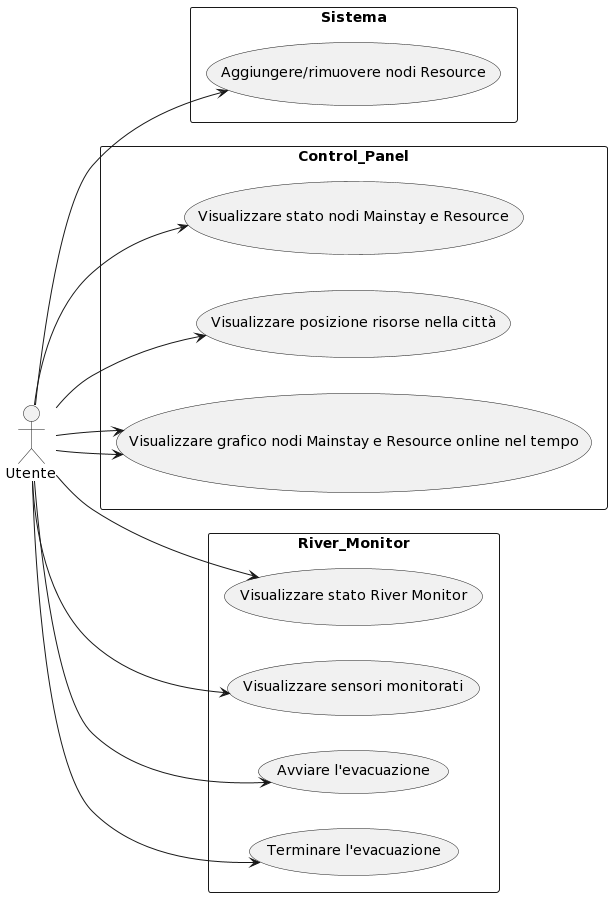
\includegraphics[width=0.8\textwidth]{../assets/images/use-cases-diagram.png}
    \label{fig:use-cases-diagram}
\end{figure}


\subsection{Requisiti Funzionali}
I requisiti funzionali delineano le funzioni specifiche del sistema, cioè cosa il sistema deve fare:
\begin{enumerate}
    \item I nodi Mainstay sono la struttura portante dell'intero sistema:
          \begin{enumerate}
              \item Ricevono informazioni dai nodi Resource che modellano sensori.
              \item Comunicano informazioni ai nodi Resource che modellano attuatori.
              \item Rilevano i malfunzionamenti dei nodi Resource.
              \item Rilevano i malfunzionamenti degli altri nodi Mainstay.
              \item Si occupano di salvare le informazioni contattando il servizio di persistenza.
              \item Non devono conoscere a prescindere le tipologie dei nodi Resource.
              \item Devono disporre di una struttura dati distribuita che permetta di memorizzare le informazioni rilevanti:
                    \begin{enumerate}
                        \item La struttura dati deve essere sincronizzata tra i nodi Mainstay.
                        \item La struttura dati deve mantenere la consistenza dei dati nel tempo.
                    \end{enumerate}
          \end{enumerate}
    \item I nodi Resource:
          \begin{enumerate}
              \item Rappresentano astrazioni di:
                    \begin{enumerate}
                        \item Sensori.
                        \item Attuatori.
                        \item Entità più complesse, come stazioni di controllo, che possono anche impiegare interfacce grafiche.
                    \end{enumerate}
              \item Fanno riferimento ad uno dei nodi Mainstay per ottenere o comunicare informazioni.
              \item Possono essere aggiunti o rimossi in tempo reale.
          \end{enumerate}
    \item Deve essere presente un servizio di persistenza dei dati che permetta di salvare in modo persistente:
          \begin{enumerate}
              \item Lo stato dei nodi Mainstay.
              \item Lo stato dei nodi Resource.
          \end{enumerate}
    \item Il malfunzionamento di un nodo non deve compromettere il funzionamento del sistema.
    \item Deve poter essere possibile introdurre nuovi moduli senza dover modificare i componenti esistenti.
    \item Vengono previsti i seguenti moduli per i nodi Resource:
          \begin{enumerate}
              \item Sensore per la rilevazione di piogge acide. Il sensore deve essere in grado di rilevare il valore di pH dell'acqua piovana, compreso tra 0 e 14.
              \item Sensore per l'analisi della qualità dell'aria. Il sensore deve essere in grado di rilevare i seguenti parametri chiave:
                    \begin{enumerate}
                        \item \label{itm:pm10} Concentrazione di PM10 (Particolato inferiore ai 10 micrometri).
                        \item \label{itm:pm25} Concentrazione di PM2,5 (Particolato inferiore ai 2,5 micrometri. Si noti che è un sottoinsieme del PM10).
                        \item \label{itm:NOx} Concentrazione di NOx (Ossidi di azoto).
                    \end{enumerate}
                    Si deve inoltre considerare che si andrà a utilizzare un sensore economico prefabbricato a basso consumo energetico, in grado di comunicare i dati rilevati tramite un protocollo di rete.
              \item Sensore per la rilevazione dell'inquinamento acustico, con le seguenti caratteristiche:
                    \begin{enumerate}
                        \item \label{itm:dB} Le letture devono variare in un intervallo di valori rappresentativi di un ambiente urbano, da 40 a 100 decibel (dB).
                        \item \label{itm:dBDescription} Oltre al valore in decibel, il sensore deve fornire una descrizione corrispondente al livello di rumore.
                    \end{enumerate}
              \item Modulo per la rilevazione del livello dell'acqua di un fiume e possibilità di intervento:
                    \begin{enumerate}
                        \item Sensore per la rilevazione degli allagamenti: il sensore deve periodicamente misurare il livello dell'acqua e comunicare il valore rilevato al nodo Mainstay.
                        \item Pannello di controllo per l'intervento in caso di allagamento, con le seguenti caratteristiche:
                              \begin{enumerate}
                                  \item Soglia di allagamento configurabile.
                                  \item Possibilità di controllare più sensori.
                                  \item Possibilità di assumere tre stati:
                                        \begin{itemize}
                                            \item Safe quando non c'è pericolo.
                                            \item Warned quando il livello dell'acqua supera la soglia di allagamento.
                                            \item Evacuating quando il livello dell'acqua supera la soglia di allagamento e l'utente ha premuto il pulsante di evacuazione.
                                        \end{itemize}
                                  \item Mostrare lo stato attuale del River Monitor.
                                  \item Passaggio in automatico allo stato Warned quando il valore della maggioranza dei sensori supera la soglia di allagamento.
                                  \item Possibilità di intervenire passando in stato Evacuating quando il sistema è Warned.
                                  \item Possibilità di intervenire tornando in stato Safe quando il sistema è Evacuating.
                              \end{enumerate}
                    \end{enumerate}
          \end{enumerate}
\end{enumerate}

\subsection{Requisiti Non Funzionali}
I requisiti non funzionali definiscono attributi di qualità, vincoli e proprietà generali del sistema:
\begin{enumerate}
    \item Affidabilità: L'affidabilità e la resilienza sono due aspetti cruciali del sistema "CityTwin". In caso di guasti hardware o malfunzionamenti dei nodi, il sistema deve essere in grado di mantenere la continuità delle operazioni fondamentali. A tale scopo, è prevista l'implementazione di un meccanismo di ridondanza, in cui i dati sono presenti in più istanze di nodi Mainstay.
    \item Performance: Il sistema deve rispondere tempestivamente alle richieste dell'utente e gestire grandi quantità di dati in tempo reale.
    \item Modularità: Il sistema deve essere realizzato in moduli separati, in modo da poter essere facilmente estendibile.
\end{enumerate}

\subsection{Requisiti di Implementazione}
I requisiti di implementazione riguardano gli aspetti tecnologici e metodologici dell'implementazione del sistema:
\begin{enumerate}
    \item Linguaggio di Programmazione: Il sistema deve essere realizzato utilizzando il linguaggio Scala 3.
    \item Architettura Basata su Attori: L'implementazione deve seguire il paradigma ad attori utilizzando il framework Akka per gestire l'interazione tra i nodi.
    \item Tecnologie di Persistenza: Il modulo di persistenza dei dati deve essere implementato utilizzando MongoDB per garantire la memorizzazione affidabile dei dati rilevati.
    \item Documentazione del Codice: Il codice deve essere adeguatamente documentato per consentire una comprensione chiara e agevolare la manutenzione futura.
\end{enumerate}


\newpage


%----------------------------------------------------------------------------------------
%	PROGETTAZIONE
%----------------------------------------------------------------------------------------

\section{Progettazione}

L'architettura del sistema, presentata in Figura \ref{fig:core-component-diagram}, è organizzata intorno a componenti interconnessi che consentono il monitoraggio e la gestione delle entità presenti all'interno della città. Ogni componente svolge ruoli specifici all'interno del sistema e interagisce attraverso interfacce ben definite.

\subsection{Suddivisione dei Componenti}

\subsubsection{Core}
Il componente centrale del sistema è il \textit{Core}, responsabile della gestione dell'elaborazione dati, del coordinamento delle attività e della comunicazione tra gli altri componenti. Il Core funge da mediatore tra le varie risorse presenti all'interno della città, ricevendo dati dai sensori e inviandoli al servizio di persistenza.

\subsubsection{Componenti Monitor}
I diversi monitor ambientali, come l'\textit{Acid Rain Monitor}, l'\textit{Air Quality Monitor}, il \textit{Noise Pollution Monitor} e il \textit{River Monitor}, costituiscono le fonti primarie di dati. Ciascun monitor raccoglie misurazioni specifiche e invia queste informazioni al \textit{Core} tramite l'interfaccia \textit{Resource}. Questa comunicazione consente al \textit{Core} di elaborare i dati e fornire una visione completa delle condizioni ambientali.

\subsubsection{Control Panel}
Il \textit{Control Panel} è l'interfaccia utente principale attraverso cui gli utenti interagiscono con il sistema. Comunica con il \textit{Core} per ottenere dati sullo stato ambientale e sul sistema nel suo complesso. Inoltre, il pannello di controllo richiede al servizio di persistenza lo storico dei dati in modo da poterli elaborare per ottenere delle statistiche.

\subsubsection{Persistence Service}
Il \textit{Persistence Service} gestisce la persistenza dei dati nel sistema. Comunica con il \textit{Core} attraverso le interfacce \textit{Post Resource} e \textit{Post Mainstay} per ricevere e salvare i dati relativi alle risorse. Analogamente, le interfacce \textit{Get Mainstay} e \textit{Get Resource }consentono di richiedere i dati al servizio di persistenza.

\begin{figure}[H]
    \caption{Diagramma dei componenti del sistema e delle loro dipendenze.}
    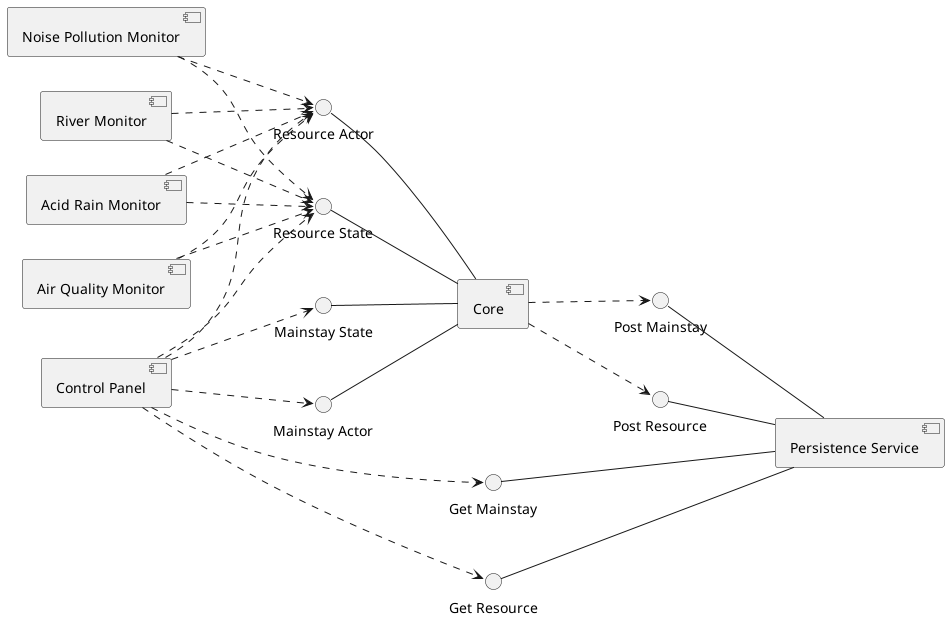
\includegraphics[width=\textwidth]{../assets/images/core-component-diagram.png}
    \label{fig:core-component-diagram}
\end{figure}

In Figura \ref{fig:nodes-component-diagram} viene presentata l'architettura dei componenti in esecuzione e dei protocolli di rete utilizzati. Il sistema è costituito da un insieme di nodi \textit{Mainstay} e \textit{Resource} che comunicano tra loro attraverso il protocollo \textit{Akka}. Inoltre, i nodi \textit{Mainstay} comunicano con il servizio di persistenza attraverso il protocollo \textit{HTTP}.
I nodi che comunicano utilizzando il protocollo \textit{Akka} sono \textit{Actor System} organizzati in un cluster, in modo da poter garantire la scalabilità del sistema.

\begin{figure}[H]
    \caption{Diagramma dei componenti in esecuzione e dei protocolli di rete utilizzati.}
    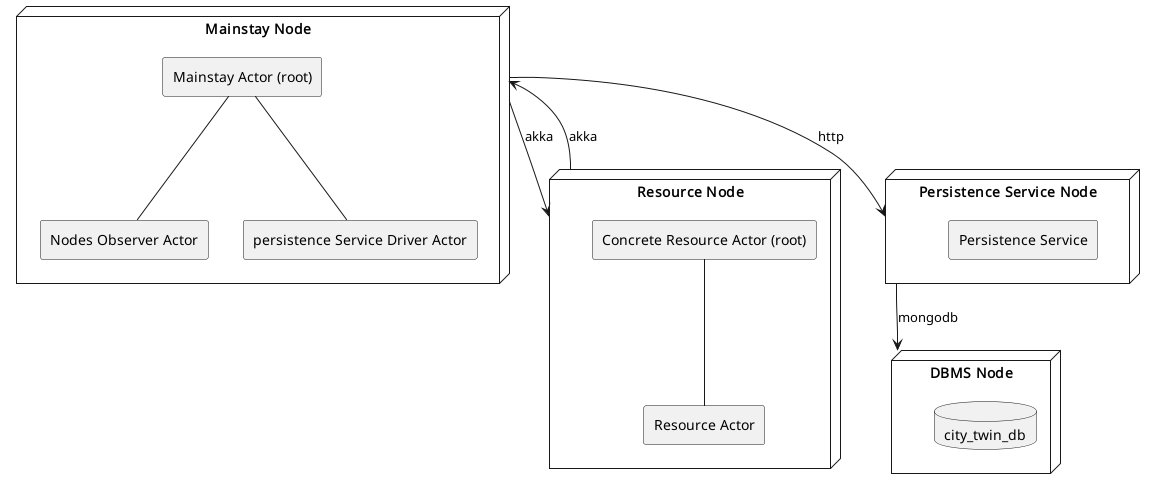
\includegraphics[width=\textwidth]{../assets/images/nodes-component-diagram.png}
    \label{fig:nodes-component-diagram}
\end{figure}

\subsection{Architettura del Modulo Core}

L'architettura del modulo \textit{Core} (Figura \ref{fig:core-class-diagram}) è costituita da diversi attori, ognuno dei quali svolge un ruolo specifico nel processo di acquisizione, gestione e comunicazione dei dati relativi alle risorse.

\textit{Resource Actor} è responsabile della gestione della risorsa, indipendentemente dal fatto che essa sia un sensore o un attuatore. Comunica con il \textit{Mainstay Actor} per ottenere o mandare lo stato delle risorse. È in grado di ricevere comandi e cambiamenti relativi alle risorse.

Il \textit{Mainstay Actor} si occupa di tenere in piedi l'intero sistema distribuito. Esso scambia lo stato delle risorse con il \textit{Resource Actor} e comunica con il \textit{Persistence Service Driver Actor} per salvare i dati nel servizio di persistenza. Inoltre, il \textit{Mainstay Actor} è responsabile della sincronizzazione dei nodi \textit{Mainstay}.

Il \textit{Nodes Observer Actor} monitora gli stati dei nodi all'interno del sistema e aggiorna il \textit{Mainstay Actor} sulla base del cambiamento di stato dei nodi.

L'attore \textit{Persistence Service Driver} è responsabile della gestione delle operazioni di persistenza dei dati. Comunica con il \textit{Mainstay Actor} per pubblicare nuovi dati al servizio di persistenza.

L'architettura prevede interazioni chiare e ben definite tra gli attori attraverso l'utilizzo di comandi specifici.

Il \textit{Resource Actor} comunica con il \textit{Mainstay Actor} utilizzando comandi come \textit{AskResourcesState}, \textit{AskAllResourcesState} e \textit{UpdateResources}. Queste interazioni consentono al \textit{Resource Actor} di ottenere informazioni sullo stato delle risorse e di aggiornare lo stato stesso.

Il \textit{Mainstay Actor} comunica con il \textit{Persistence Service Driver Actor} utilizzando comandi come \textit{PostMainstay} e \textit{PostResource}. Queste interazioni consentono al \textit{Mainstay Actor} di inviare nuovi dati al servizio di persistenza.

\begin{figure}[H]
    \caption{Diagramma delle classi del modulo \textit{Core}.}
    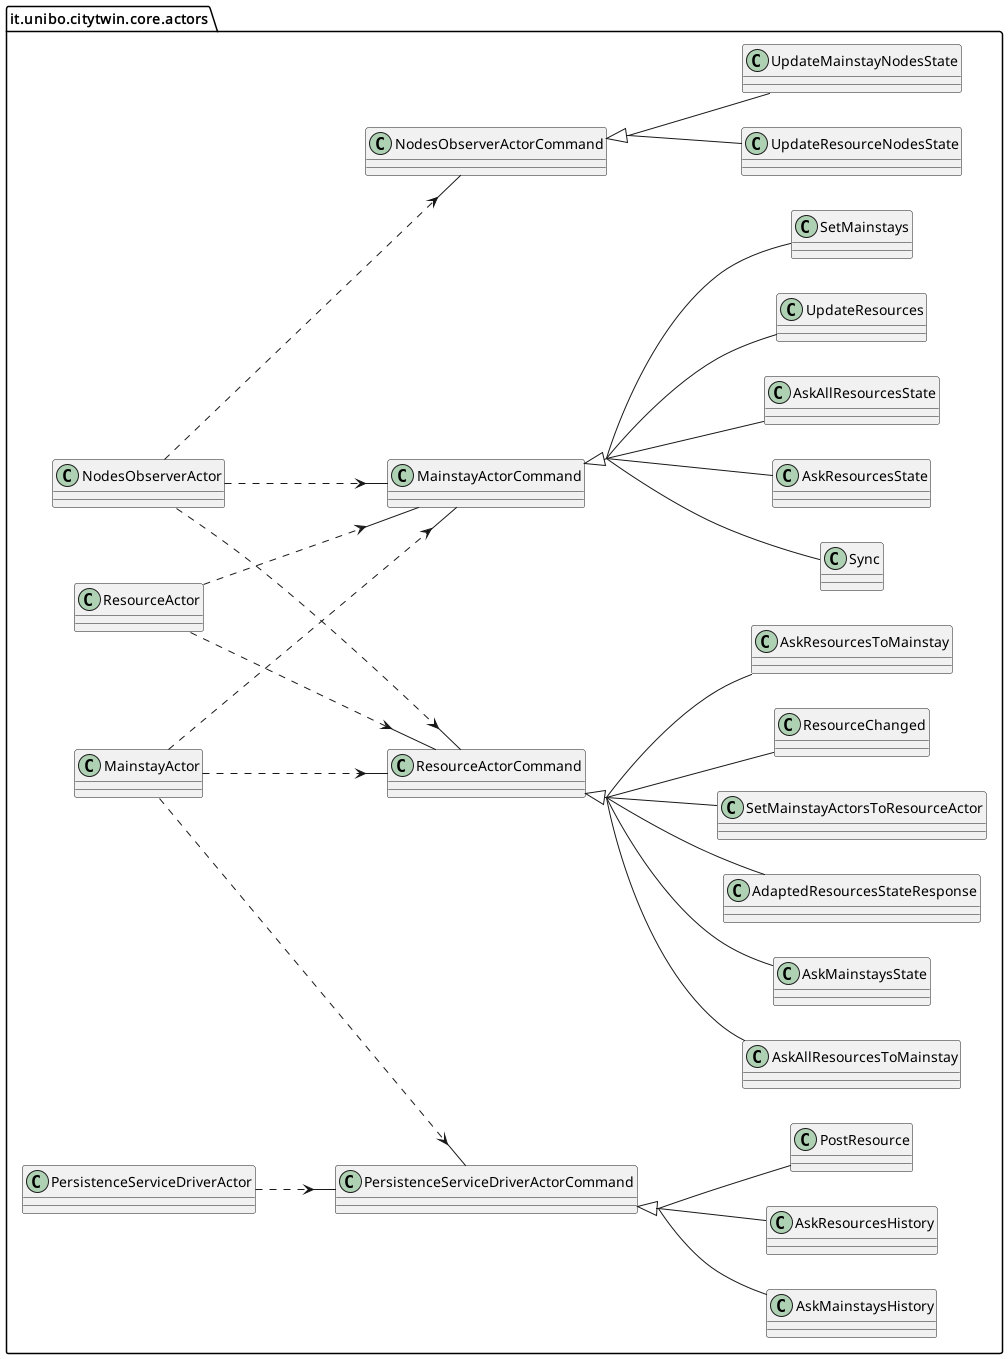
\includegraphics[width=\textwidth]{../assets/images/core-class-diagram.png}
    \label{fig:core-class-diagram}
\end{figure}

\subsection{Definizione delle Interazioni dei Componenti}

Il comportamento generale del sistema viene definito sulla base di una serie di interazioni tra i componenti. In particolare, le interazioni possono essere raggruppate per definire un determinato aspetto di tale comportamento.

\subsubsection{Aggiornamento Sullo Stato dei Nodi}

Lo scambio di messaggi tra \textit{Nodes Observer Actor} e \textit{Mainstay Actor} (Figura \ref{fig:core-nodes-state-sequence-diagram}) è volto a mantenere aggiornato quest'ultimo sullo stato generale dei nodi del sistema. Nel momento in cui il \textit{Mainstay Actor} riceve un aggiornamento sui nodi, esso aggiorna il proprio stato e lo comunica al \textit{Persistence Service Driver Actor}, che si occupa di rendere persistenti i dati tramite il servizio di persistenza.

\begin{figure}[H]
    \caption{Diagramma di sequenza per l'aggiornamento sullo stato dei nodi del sistema.}
    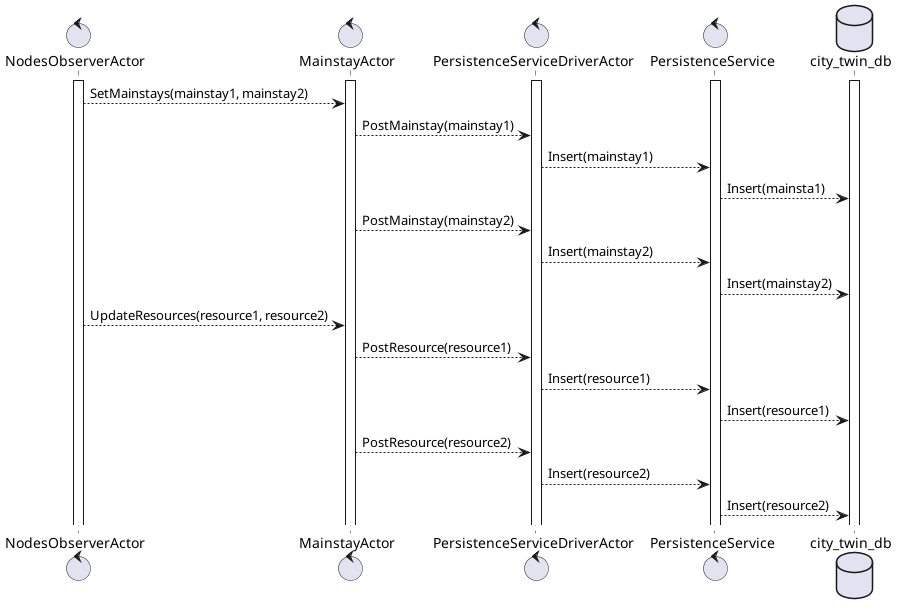
\includegraphics[width=\textwidth]{../assets/images/core-nodes-state-sequence-diagram.png}
    \label{fig:core-nodes-state-sequence-diagram}
\end{figure}

\subsubsection{Aggiornamento Sullo Stato delle Risorse}

Lo scambio di messaggi tra \textit{Resource Actor} e \textit{Mainstay Actor} (Figura \ref{fig:core-resource-state-exchange-sequence-diagram}) è utile a:
\begin{itemize}
    \item Ottenere lo stato delle altre risorse e comunicare il proprio nel caso un cui il nodo \textit{Resource} modella un attuatore.
    \item Comunicare lo stato della risorsa nel caso un cui il nodo \textit{Resource} modella un sensore.
\end{itemize}

In ogni caso, quando il \textit{Mainstay Actor} riceve un aggiornamento, lo comunica al servizio di persistenza tramite il \textit{Persistence Service Driver Actor}.

\begin{figure}[H]
    \caption{Diagramma di sequenza per lo scambio dello stato delle risorse.}
    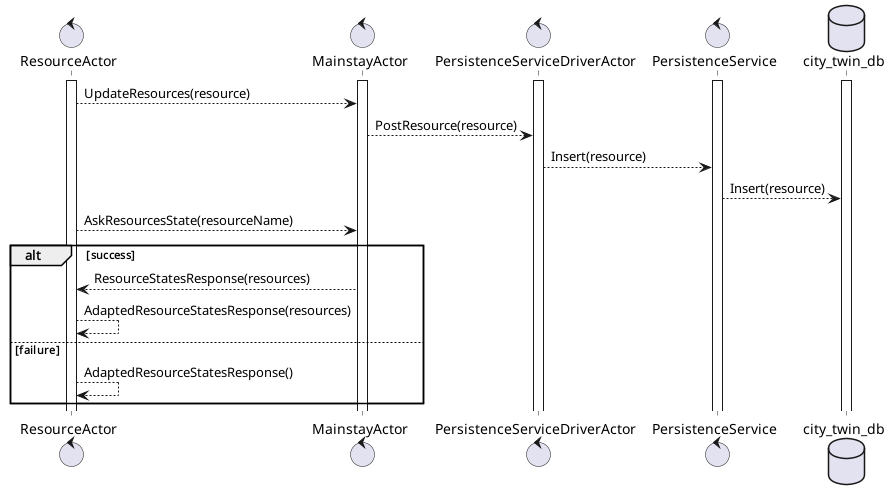
\includegraphics[width=\textwidth]{../assets/images/core-resource-state-exchange-sequence-diagram.png}
    \label{fig:core-resource-state-exchange-sequence-diagram}
\end{figure}

\subsubsection{Sincronizzazione dei Nodi Mainstay}

Come detto precedentemente, i nodi \textit{Mainstay} sono i pilastri portanti dell'intero sistema e si occupano della gestione dei dati riguardanti le risorse e i nodi. I nodi \textit{Mainstay} devono essere sempre sincronizzati tra loro, in modo da poter garantire la coerenza dei dati. Per questo motivo, i nodi \textit{Mainstay} si sincronizzano ogni volta che una risorsa manda il suo stato ad uno di questi. In Figura \ref{fig:core-mainstays-sync-sequence-diagram} viene presentato il diagramma di sequenza per la sincronizzazione dei nodi \textit{Mainstay}.

\begin{figure}[H]
    \caption{Diagramma di sequenza per la sincronizzazione dei nodi Mainstay.}
    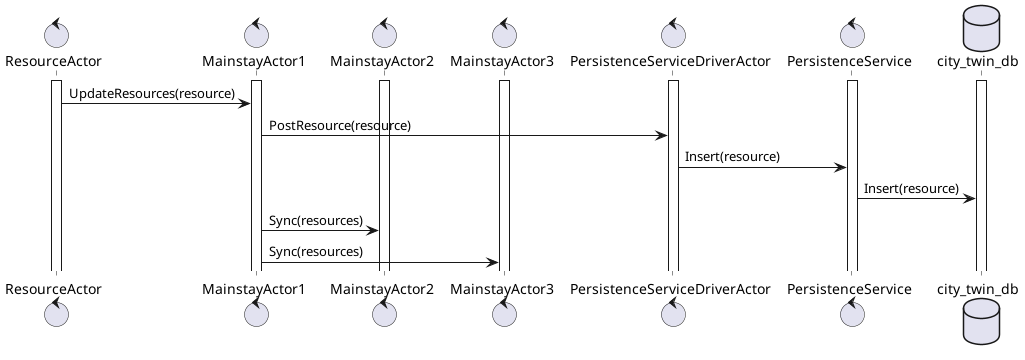
\includegraphics[width=\textwidth]{../assets/images/core-mainstays-sync-sequence-diagram.png}
    \label{fig:core-mainstays-sync-sequence-diagram}
\end{figure}

\subsubsection{Aggiornamento del Pannello di Controllo}

Il comportamento del \textit{Control Panel} (Figura \ref{fig:control-panel-sequence-diagram}) viene modellato come un caso particolare di risorsa che comunica con il \textit{Mainstay Actor} per ottenere lo stato delle risorse e dei nodi. Inoltre, il \textit{Control Panel} comunica con il servizio di persistenza per ottenere lo storico dei dati e calcolare le statistiche.

\begin{figure}[H]
    \caption{Diagramma di sequenza per l'aggiornamento del pannello di controllo.}
    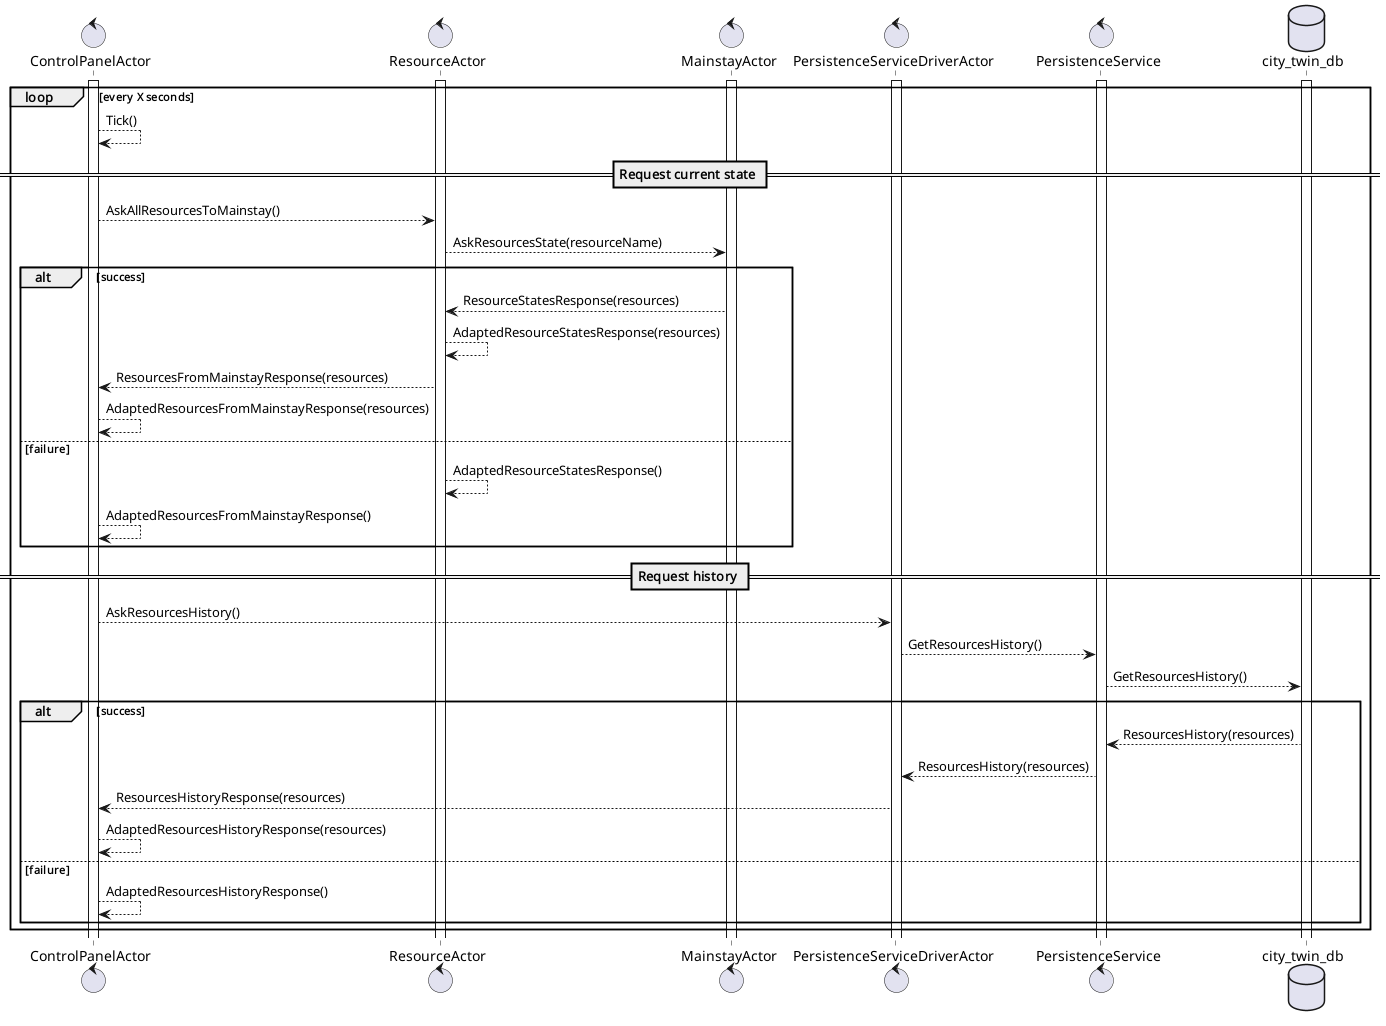
\includegraphics[width=\textwidth]{../assets/images/control-panel-sequence-diagram.png}
    \label{fig:control-panel-sequence-diagram}
\end{figure}

\subsection{Progettazione dei Moduli Monitor}
I componenti monitor sono elementi fondamentali del sistema, in quanto raccolgono dati ambientali cruciali per valutare le condizioni della città. Ogni componente monitor è progettato per monitorare un aspetto specifico dell'ambiente, come la qualità dell'aria, la presenza di inquinamento acustico, il livello dell'acqua dei fiumi e i livelli di acidità delle piogge. Di seguito verranno forniti dettagli su ciascun componente monitor.

\subsubsection{Acid Rain Monitor}
Le piogge acide sono fenomeni meteorologici caratterizzati dall'acidificazione delle precipitazioni atmosferiche, come pioggia o neve, a causa dell'elevato contenuto di sostanze acide, in particolare anidride solforosa ed ossidi di azoto, nell'atmosfera. Questi agenti inquinanti vengono principalmente prodotti da processi industriali e veicolari. Le piogge acide possono causare seri danni agli ecosistemi, alle coltivazioni agricole, agli edifici e alle infrastrutture, oltre a influire negativamente sulla qualità dell'acqua nei corsi d'acqua e nei laghi.

\paragraph{Obiettivo e Scopo}
Il principale scopo dell'Acid Rain Monitor è monitorare i livelli di pH delle piogge acide per rilevare eventuali situazioni di acidificazione dell'ambiente. Questo componente fornisce informazioni utili per valutare l'impatto delle piogge acide e prendere eventuali misure correttive.

\paragraph{Caratteristiche}
L'Acid Rain Monitor è rappresentato da un \textit{Acid Rain Sensor}, identificato da un nome univoco e una posizione geografica. Il sensore è in grado di rilevare il livello di pH dell'acqua piovana. Il range di valori che può rilevare varia da 0 a 14, dove 0 indica una forte acidità, 7 indica neutralità e 14 indica un'elevata alcalinità. Il sensore effettua rilevamenti periodici per monitorare i cambiamenti nei livelli di pH nel tempo.

\paragraph{Architettura}
L'architettura dell'Acid Rain Monitor prevede una stretta collaborazione con il \textit{Resource Actor}, un componente principale del sistema. L'\textit{Acid Rain Sensor} genera periodicamente un messaggio di \textit{tick} verso se stesso, il quale avvia il processo di rilevamento del pH. Una volta ottenuto il valore del pH, il sensore invia questo dato al \textit{Resource Actor}, che si occupa di comunicare i dati al \textit{Mainstay Actor}.

\paragraph{Interazione con il Resource Actor}
Il sensore interagisce con il \textit{Resource Actor} attraverso l'invio di dati relativi ai rilevamenti del pH. Il sensore invia al \textit{Resource Actor} un messaggio contenente il valore del pH e altre informazioni come il nome e la sua posizione. Il \textit{Resource Actor} comunica e invia i dati direttamente al \textit{Mainstay Actor}, rendendoli disponibili per le diverse parti del sistema che richiedono informazioni sui rilevamenti. In Figura \ref{fig:sensor-resourceactor-interaction-diagram} viene presentato il diagramma di sequenza per l'interazione tra il sensore dell'Acid Rain Monitor e il \textit{Resource Actor}.

\begin{figure}[H]
    \centering
    \caption{Diagramma di sequenza per l'interazione tra un sensore e il relativo \textit{Resource Actor}.}
    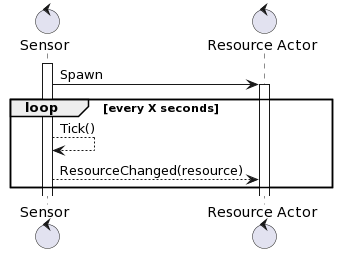
\includegraphics[width=0.6\textwidth]{../assets/images/sensor-resourceactor-interaction-diagram.png}
    \label{fig:sensor-resourceactor-interaction-diagram}
\end{figure}

\subsubsection{Air Quality Monitor}
L'Air Quality Monitor è progettato per monitorare la qualità dell'aria, fornendo informazioni sulle concentrazioni di particelle sottili (PM10 e PM2.5) e ossidi di azoto (NOx). La qualità dell'aria è un aspetto critico dell'ambiente urbano, influenzando la salute delle persone, la vegetazione e la qualità complessiva della vita in città. Livelli elevati di PM10, PM2.5 e NOx sono associati a problemi respiratori, malattie cardiache e impatti negativi sull'ambiente.

\paragraph{Obiettivo e Scopo}
Il principale scopo dell'Air Quality Monitor è monitorare i livelli di PM10, PM2.5 e NOx nell'aria circostante, al fine di valutare la qualità dell'aria e identificare situazioni di inquinamento atmosferico. Questo componente fornisce dati cruciali per valutare il livello di inquinamento dell'aria e prendere decisioni per mitigare gli effetti negativi.

\paragraph{Caratteristiche}
L'Air Quality Monitor è costituito da un \textit{Air Sensor}, caratterizzato da un nome univoco e una posizione geografica. Il sensore è in grado di rilevare i parametri indicati dai requisiti \ref{itm:pm10}, \ref{itm:pm25} e \ref{itm:NOx} nell'aria circostante.

\paragraph{Architettura}
Come nel caso dell'Acid Rain Monitor, l'Air Quality Monitor prevede una stretta collaborazione con il \textit{Resource Actor}. L'\textit{Air Sensor} simula il comportamento del sensore, effettuando rilevamenti periodici dei livelli di PM10, PM2.5 e NOx comunicando con sensore fisico tramite un protocollo di rete. I dati rilevati vengono quindi inviati al \textit{Resource Actor}, che si occupa di comunicarli al \textit{Mainstay Actor} per l'archiviazione e l'accesso ai dati.

\paragraph{Interazione con il Resource Actor}
Il sensore interagisce con il \textit{Resource Actor} attraverso l'invio di dati relativi ai parametri chiave della qualità dell'aria. Il sensore invia al \textit{Resource Actor} un messaggio contenente i valori dei parametri chiave e altre informazioni come il nome e la sua posizione. Il \textit{Resource Actor} comunica e invia i dati direttamente al \textit{Mainstay Actor}, rendendoli disponibili per le diverse parti del sistema che richiedono informazioni sui rilevamenti. In Figura \ref{fig:sensor-resourceactor-interaction-diagram} viene presentato il diagramma di sequenza per l'interazione tra il sensore dell'Air Quality Monitor e il \textit{Resource Actor}.

\subsubsection{Noise Pollution Monitor}
L'inquinamento acustico è un problema urbano che può avere effetti negativi sulla salute umana, sull'ambiente e sulla qualità della vita complessiva. I livelli elevati di rumore possono causare disturbi al sonno, stress, problemi uditivi e disturbi della concentrazione. Il Noise Pollution Monitor è progettato per misurare e monitorare i livelli di rumore nell'ambiente circostante, al fine di valutare l'inquinamento acustico e identificare situazioni critiche.

\paragraph{Obiettivo e Scopo}
L'obiettivo principale del Noise Pollution Monitor è rilevare il livello di rumore nell'area circostante e fornire una valutazione della situazione di inquinamento acustico. Questo componente fornisce dati essenziali per comprendere l'entità del problema e adottare misure per mitigare gli effetti negativi del rumore.

\paragraph{Caratteristiche}
Il Noise Pollution Monitor è rappresentato da un \textit{Noise Sensor}, identificato da un nome univoco e una posizione geografica. È in grado di misurare i livelli di rumore espressi in decibel (dB), con un range tipico di 40 dB (ambiente tranquillo) a 100 dB (ambiente molto rumoroso) e fornire la corrispondente descrizione, come indicato dai requisiti \ref{itm:dB} e \ref{itm:dBDescription}. Il sensore effettua rilevamenti periodici dei livelli di rumore.

\paragraph{Architettura}
Come nel caso dell'Acid Rain Monitor e dell'Air Quality Monitor, il Noise Pollution Monitor prevede una stretta collaborazione con il \textit{Resource Actor}. Il \textit{Noise Sensor} genera periodicamente un messaggio di \textit{tick} verso se stesso, responsabile di simulare il comportamento del sensore di rumore. Una volta ottenuti i dati, il sensore invia questi dati al \textit{Resource Actor}, che si occupa di comunicare i dati al \textit{Mainstay Actor}.

\paragraph{Interazione con il Resource Actor}
Il \textit{Noise Sensor} interagisce con il \textit{Resource Actor} attraverso lo scambio di risorse contenenti i dati del rilevamento del rumore. Il \textit{Noise Sensor} crea una risorsa che include il valore di livello di rumore misurato e una descrizione corrispondente al livello di rumore. Questa risorsa viene inviata al \textit{Resource Actor}, che la comunica al \textit{Mainstay Actor}. Da qui, i dati possono essere accessibili da altre parti del sistema che richiedono informazioni sui rilevamenti. Il diagramma di sequenza in Figura \ref{fig:sensor-resourceactor-interaction-diagram} illustra l'interazione tra il sensore di inquinamento acustico e il \textit{Resource Actor}.

\subsubsection{River Monitor}
Il "River Monitor" è un complesso sistema progettato per rilevare, monitorare e rispondere alle situazioni di alluvione in aree sensibili. Questa sezione descrive in dettaglio il design concettuale del sistema, delineando i componenti chiave e il loro ruolo all'interno dell'architettura complessiva.

\paragraph{Architettura}
Nel sistema sistema di monitoraggio del fiume sono presenti i seguenti nodi \textit{Resource}, i quali non comunicano quindi direttamente tra di loro ma ognuno attraverso il proprio \textit{Resource Actor}:

\begin{enumerate}
    \item \textbf{Flood Sensor}: I sensori di alluvione costituiscono il primo punto di contatto con l'ambiente circostante. Rilevano costantemente i livelli dell'acqua e comunicano i dati al \textit{Resource Actor} corrispondente. Questa interazione è illustrata nel diagramma di sequenza in Figura \ref{fig:sensor-resourceactor-interaction-diagram}.

    \item \textbf{River Monitor Actor}: Il \textit{River Monitor} è un componente centrale del sistema. Ha il compito di monitorare i dati provenienti dai sensori di alluvione, valutare le condizioni correnti e prendere decisioni in base ai dati ricevuti. Il \textit{River Monitor} può attivare allarmi e avviare procedure di evacuazione. Per rappresentare lo stato del \textit{River Monitor} è stato introdotto il \textit{River Monitor State Actor}, il quale riceve messaggi dal \textit{River Monitor Actor} riguardo ai cambiamenti di stato, come la necessità di passare in stato di allarme o il passaggio allo stato di evacuazione. Il diagramma di sequenza in Figura \ref{fig:rivermonitor-resourceactor-interaction-diagram} illustra l'interazione tra il \textit{River Monitor Actor}, il \textit{River Monitor State Actor} e il \textit{Resource Actor}.

    \item \textbf{View}: La \textit{View} rappresenta l'interfaccia utente dell'applicazione. Fornisce una rappresentazione visiva dello stato del \textit{River Monitor} e consente agli utenti di interagire con il sistema. Gli utenti possono visualizzare lo stato corrente, avviare procedure di evacuazione o segnalare zone come "evacuate" dopo aver avviato l'evacuazione. Nel diagramma di sequenza in Figura \ref{fig:view-interaction-diagram} viene illustrata l'interazione tra la \textit{View}, il \textit{View Actor} e il \textit{Resource Actor}.
\end{enumerate}

\begin{figure}[H]
    \caption{Diagramma di sequenza per l'interazione tra River Monitor Actor, River Monitor State Actor e Resource Actor.}
    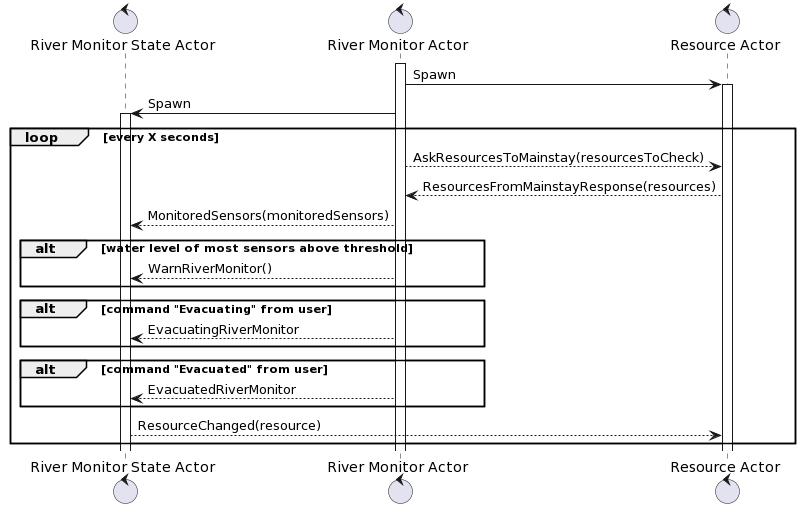
\includegraphics[width=\textwidth]{../assets/images/rivermonitor-resourceactor-interaction-diagram.png}
    \label{fig:rivermonitor-resourceactor-interaction-diagram}
\end{figure}

\begin{figure}[H]
    \caption{Diagramma di sequenza per l'interazione tra View, View Actor e Resource Actor.}
    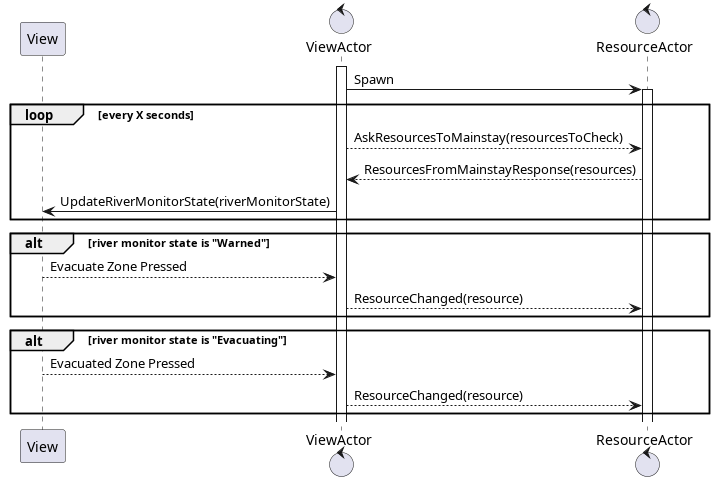
\includegraphics[width=\textwidth]{../assets/images/view-interaction-diagram.png}
    \label{fig:view-interaction-diagram}
\end{figure}

\paragraph{Flusso di Lavoro}

Il flusso di lavoro all'interno del sistema di monitoraggio del fiume è il seguente:

\begin{enumerate}
    \item I sensori di alluvione rilevano continuamente i livelli dell'acqua e inviano i dati al \textit{Resource Actor}.

    \item Il \textit{River Monitor Actor} richiede al \textit{Resource Actor} lo stato delle risorse che sta monitorando, ovvero i sensori e la view. In condizioni normali, il \textit{River Monitor} è in stato \textit{Safe}.

    \item Il \textit{River Monitor Actor} valuta le misurazioni dei sensori per determinare se è necessario passare allo stato di allarme. Nello specifico, comunica al \textit{River Monitor State Actor} di passare allo stato di \textit{Warned} se il livello dell'acqua della maggior parte dei sensori supera una soglia critica.

    \item Il \textit{River Monitor Actor} controlla le risorse relative alla view perché se l'utente ha avviato una procedura di evacuazione (possibile solo se il \textit{River Monitor State Actor} è in stato di allarme), il \textit{River Monitor State Actor} cambia il suo stato in \textit{Evacuating}. dallo stato di \textit{Evacuating} il \textit{River Monitor State Actor} può passare allo stato di \textit{Evacuated} se l'utente ha segnalato che la zona è stata evacuata. in questo caso il \textit{River Monitor State Actor} torna allo stato \textit{Safe}.

    \item A questo punto il \textit{River Monitor State Actor} comunica al \textit{Resource Actor} il suo stato e i sensori monitorati, in modo che queste informazioni possano essere visualizzate nella \textit{View}.

    \item La \textit{View} visualizza lo stato corrente del \textit{River Monitor} agli utenti e consente loro di agire, avviando procedure di evacuazione e di fine evacuazione quando lo stato del \textit{River Monitor} lo consente.
\end{enumerate}

\newpage

%----------------------------------------------------------------------------------------
%	IMPLEMENTAZIONE
%----------------------------------------------------------------------------------------

\section{Implementazione}\label{sec:implementazione}

\subsection{Tecnologie Utilizzate}

\subsubsection{Scala 3}

Scala 3 è una versione successiva del linguaggio di programmazione Scala, progettato per migliorare e semplificare ulteriormente l'esperienza di programmazione funzionale e orientata agli oggetti. È un linguaggio staticamente tipizzato che unisce caratteristiche provenienti da diversi paradigmi di programmazione, consentendo agli sviluppatori di scrivere codice conciso ed elegante mentre sfruttano la potenza dei tipi statici.

\subsubsection{Simple Build Tool (SBT)}

SBT è uno strumento di build e gestione delle dipendenze ampiamente utilizzato nella comunità di sviluppo software in linguaggio Scala. È stato creato per semplificare il processo di compilazione, test e distribuzione delle applicazioni Scala.

Alcuni aspetti chiave di SBT:

\begin{itemize}
    \item Utilizza un DSL per definire come il progetto dovrebbe essere compilato, testato e confezionato. Questo DSL consente di specificare dettagli come le dipendenze del progetto, le task da eseguire e le configurazioni di compilazione.
    \item È altamente personalizzabile tramite l'uso di plugin. Esistono numerosi plugin disponibili per SBT che estendono le sue funzionalità, ad esempio per l'integrazione con strumenti di continuous integration, per la generazione di documentazione automatica o per l'integrazione con framework di testing.
    \item Supporta la gestione di progetti multi-progetto, in cui più sotto-progetti possono condividere dipendenze e risorse comuni. Questo è particolarmente utile quando si lavora su sistemi software complessi composti da più moduli o componenti.
\end{itemize}

\subsubsection{Akka}

Akka è un toolkit open-source scritto in Scala che offre un modello di programmazione per costruire applicazioni distribuite, concorrenti e reattive basate su attori. Gli attori sono unità fondamentali di elaborazione in Akka e rappresentano entità concorrenti leggere che comunicano tra loro attraverso messaggi. Questo modello di programmazione facilita la gestione dell'elaborazione parallela e distribuita in modo efficiente.

Alcuni concetti chiave all'interno del toolkit Akka:

\begin{itemize}
    \item Attori: Gli attori sono la base del modello di programmazione in Akka. Ogni attore è una singola unità di elaborazione che può ricevere messaggi, eseguire calcoli e inviare messaggi ad altri attori. Gli attori sono isolati e indipendenti, il che semplifica la gestione dei thread e delle risorse concorrenti.
    \item Sistema di attori: Akka fornisce un sistema di attori che gestisce l'allocazione e la comunicazione degli attori. Il sistema di attori si occupa della gestione dei thread, del ciclo di vita degli attori e delle loro comunicazioni asincrone attraverso l'invio di messaggi.
    \item Modello di messaggistica: In Akka, gli attori comunicano inviando messaggi asincroni. Questo modello di messaggistica facilita la creazione di applicazioni reattive in cui gli attori possono rispondere in modo efficiente ai messaggi ricevuti senza bloccare l'elaborazione.
    \item Supervisione e gerarchia degli attori: Gli attori possono essere organizzati in una gerarchia, dove gli attori genitori supervisionano il comportamento dei loro figli. Questo consente una maggiore resilienza, in quanto gli errori in un attore possono essere gestiti in modo gerarchico, consentendo il ripristino o la terminazione controllata degli attori falliti.
    \item Sistemi distribuiti: Akka facilita la costruzione di sistemi distribuiti attraverso l'implementazione di attori distribuiti. Gli attori distribuiti possono esistere su nodi separati in una rete e comunicare attraverso la rete stessa, consentendo la costruzione di applicazioni scalabili e resilienti.
\end{itemize}

\subsubsection{Node.js}

Node.js\cite{nodejs} è una piattaforma open-source basata sul motore JavaScript V8 di Google, progettata per consentire l'esecuzione di codice JavaScript lato server. Prima dell'avvento di Node.js, JavaScript era principalmente utilizzato all'interno dei browser per creare interazioni dinamiche nelle pagine web. Tuttavia, Node.js ha esteso il suo utilizzo consentendo di eseguire codice JavaScript anche sul server, aprendo la strada a numerose possibilità di sviluppo web e applicativo.

Alcune delle caratteristiche chiave di Node.js:

\begin{itemize}
    \item Architettura asincrona e non bloccante: Node.js è noto per il suo modello asincrono e non bloccante, che permette di gestire molte connessioni contemporaneamente senza rallentamenti. Questo è particolarmente utile per le applicazioni in tempo reale, come le applicazioni di chat o di gioco online.
    \item Moduli: Node.js utilizza un sistema di moduli per organizzare il codice in componenti riutilizzabili. I moduli possono essere creati per separare le funzionalità in file separati, rendendo il codice più gestibile e manutenibile.
    \item NPM (Node Package Manager): NPM è un gestore di pacchetti che permette agli sviluppatori di installare, condividere e gestire librerie e pacchetti di terze parti. Questo ecosistema di pacchetti offre una vasta gamma di strumenti e librerie che semplificano lo sviluppo.
    \item Server Web: Node.js può essere utilizzato per creare server web altamente scalabili ed efficienti. Molti framework, come Express.js, sono disponibili per semplificare la creazione di applicazioni web.
\end{itemize}

\subsubsection{MongoDB}

MongoDB è un database NoSQL ampiamente utilizzato per gestire e archiviare grandi quantità di dati, inclusi dati non strutturati, semi-strutturati e strutturati. È progettato per essere flessibile, scalabile e performante, ed è particolarmente adatto per applicazioni che richiedono un'archiviazione e un accesso veloce a dati complessi e eterogenei.

\subsubsection{Docker}

Docker è una tecnologia di virtualizzazione leggera e di containerizzazione che consente di creare, distribuire e gestire applicazioni e servizi in ambienti isolati noti come "container". Questi container includono tutto ciò di cui un'applicazione ha bisogno per essere eseguita, come il codice, le librerie, le dipendenze e le variabili d'ambiente, il tutto condiviso su una base immutabile. Questo concetto di containerizzazione rende Docker un approccio efficace per sviluppare, testare e distribuire applicazioni in modo rapido e consistente su diverse piattaforme.

\subsubsection{Servizio FAAS Microsoft Azure Functions}

Il servizio Azure Functions\cite{azurefunctions} (Funzioni di Azure) è una soluzione di elaborazione serverless offerta da Microsoft Azure\cite{microsoftazure}. Questo servizio consente agli sviluppatori di scrivere, distribuire ed eseguire rapidamente codice in risposta ad eventi specifici senza preoccuparsi dell'infrastruttura sottostante. Le Azure Functions sono progettate per essere altamente scalabili e reattive, rendendole ideali per scenari in cui è richiesta una risposta rapida a eventi come richieste HTTP, scadenze temporali o trigger di database.

\subsection{Problematiche Riscontrate e Soluzioni Adottate}

\subsubsection{Serializzazione delle Strutture Dati}

La serializzazione in Akka è il processo di convertire oggetti Scala in un formato che può essere trasmesso attraverso la rete e quindi ricostruito in un oggetto equivalente. Questo è particolarmente importante in un ambiente basato su attori, in cui i messaggi vengono inviati tra attori in diversi processi o nodi. Lo scambio di messaggi prevede l'utilizzo di strutture dati, che in un sistema distribuito devono essere serializzate prima di essere inviate.

Durante il processo di sviluppo si sono presentati problemi di serializzazione delle \verb|HashMap[A, B]| (dove \verb|A| e \verb|B| sono tipi generici), per questo motivo si è scelto di convertire le \verb|HashMap[A, B]| in \verb|Set[(A, B)]| per lo scambio di messaggi tra attori.

Un altro tipo di struttura dati che non è possibile serializzare direttamente è l'enumerazione di Scala 3. Per questo motivo, si è scelto di utilizzare un'enumerazione di Scala 2, che è serializzabile.

Esempio di enumerazione in Scala 3:

\begin{lstlisting}[language=Scala]
    enum ResourceType:
        case Act
        case Sense
\end{lstlisting}

Esempio di enumerazione in Scala 2:

\begin{lstlisting}[language=Scala]
    object ResourceType extends Enumeration:
        type ResourceType = Value
        val Act, Sense = Value
\end{lstlisting}

\subsubsection{Rappresentazione dello Stato delle Risorse}

I nodi \textit{Mainstay} sono stati concepiti per essere generici e indipendenti dagli altri moduli del sistema. Per questo motivo non conoscono il tipo di risorse presenti a runtime e quindi non possono interpretarne lo stato. Questa risulta una problematica nel momento in cui lo stato della risorsa va serializzato per essere inviato ad un nodo \textit{Mainstay}.

In origine il tipo dello stato della risorsa è stato definito come \verb|Any|, ma questo ha portato a problemi di serializzazione. Per risolvere questo problema, si è scelto di tipizzare lo stato come \verb|String|, in modo che esso possa essere definito in formato JSON.

\subsection{Implementazione del Control Panel}

Il pannello di controllo è stato progettato per essere facilmente utilizzabile da qualsiasi tipo di utente. Le interazioni necessarie per visualizzare le informazioni desiderate sono state ridotte al minimo, in modo da rendere l'esperienza utente il più semplice possibile.

Il pannello di controllo dispone di quattro schermate:

\begin{itemize}
    \item \textbf{Mappa della città} (Figura \ref{fig:control-panel-map}): visualizza la posizione delle risorse nella città, indicandone il nome e lo stato (online/offline).
    \item \textbf{Pannello delle informazioni} (Figura \ref{fig:control-panel-info}): visualizza in tempo reale le informazioni sullo stato delle risorse e dei Mainstay.
    \item \textbf{Pannello delle statistiche dei nodi Resource} (Figura \ref{fig:control-panel-resources-stats}): visualizza lo stato dei nodi Resource nel tempo.
    \item \textbf{Pannello delle statistiche dei nodi Mainstay}: visualizza lo stato dei nodi Mainstay nel tempo.
\end{itemize}

\begin{figure}[H]
    \caption{Control Panel: schermata della mappa della città.}
    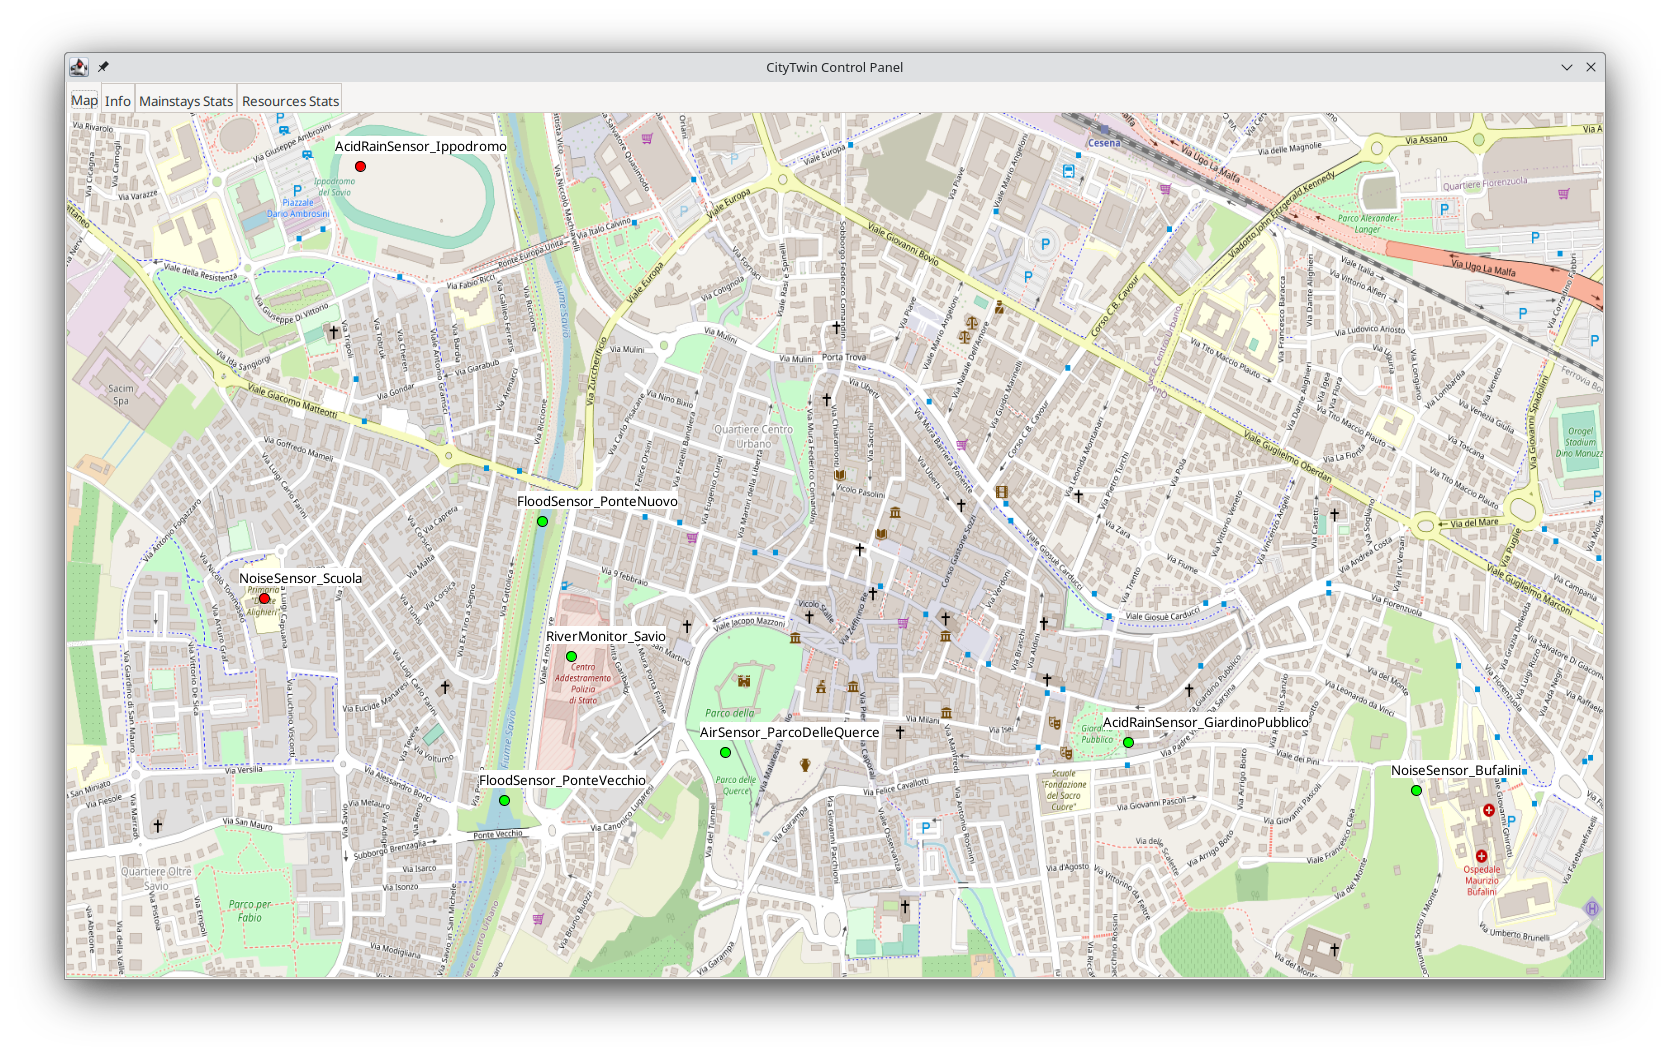
\includegraphics[width=\textwidth]{../assets/images/control-panel-map.png}
    \label{fig:control-panel-map}
\end{figure}

\begin{figure}[H]
    \caption{Control Panel: schermata delle informazioni sullo stato dei nodi \textit{Resource} e dei nodi \textit{Mainstay}.}
    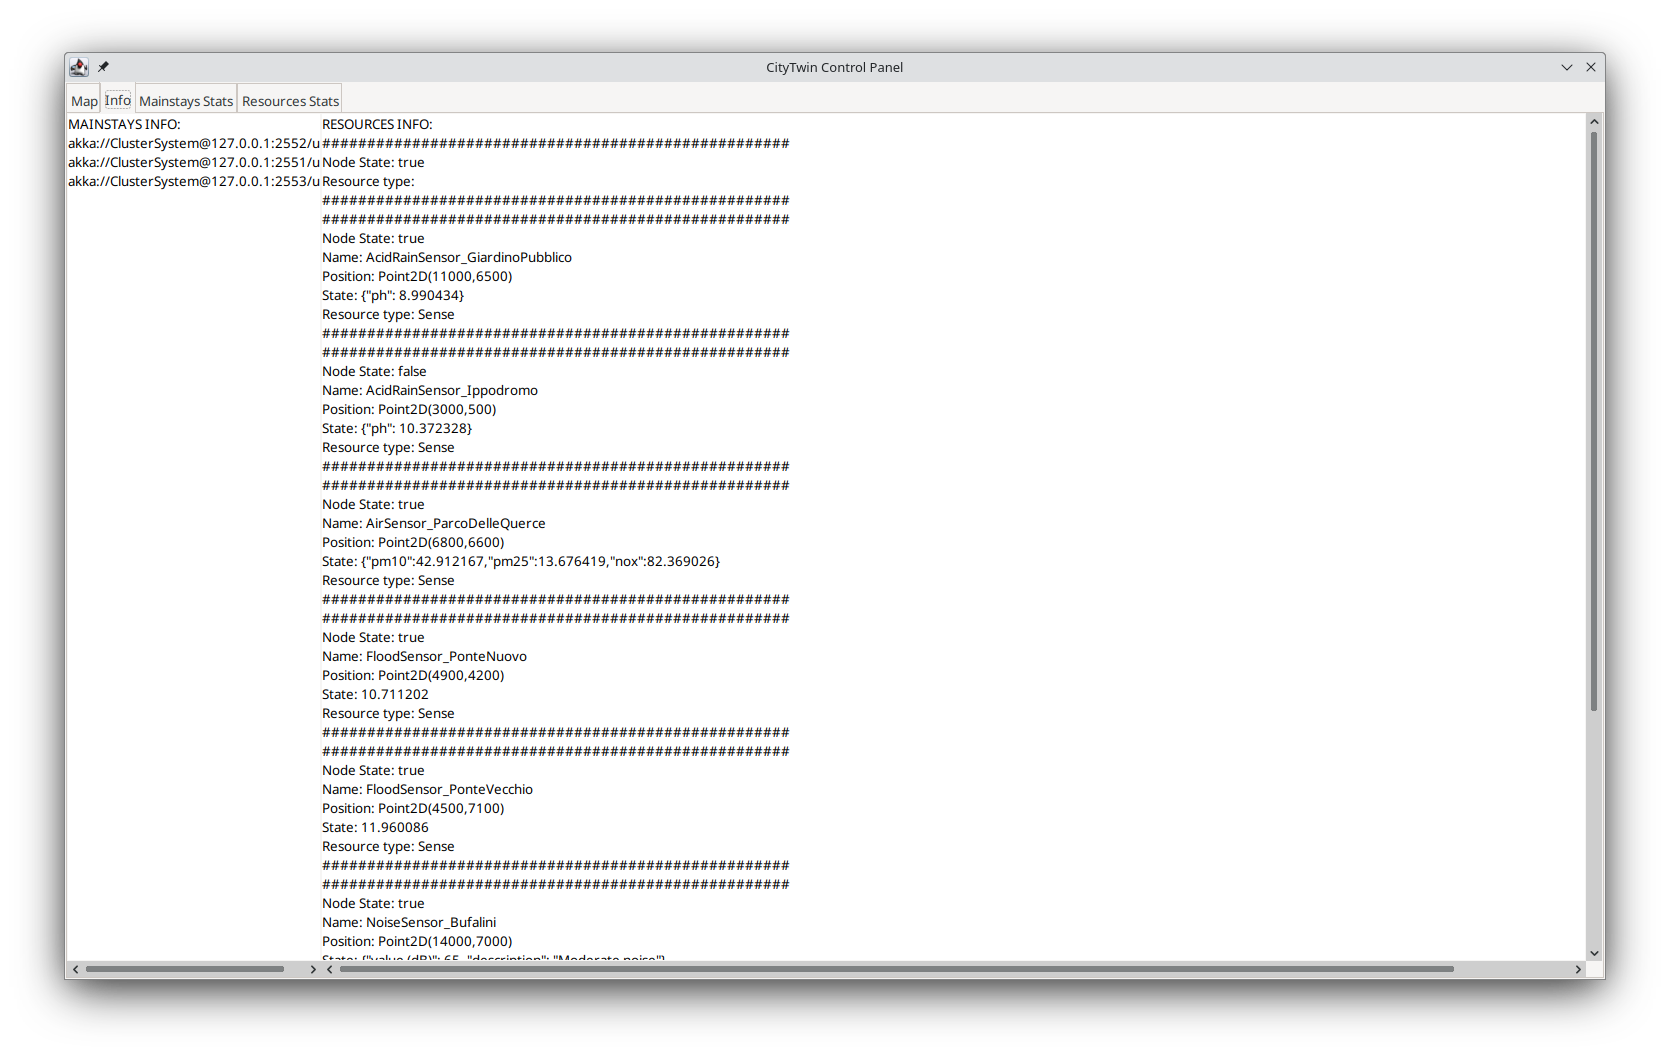
\includegraphics[width=\textwidth]{../assets/images/control-panel-info.png}
    \label{fig:control-panel-info}
\end{figure}

\begin{figure}[H]
    \caption{Control Panel: schermata delle statistiche dei nodi \textit{Resource}.}
    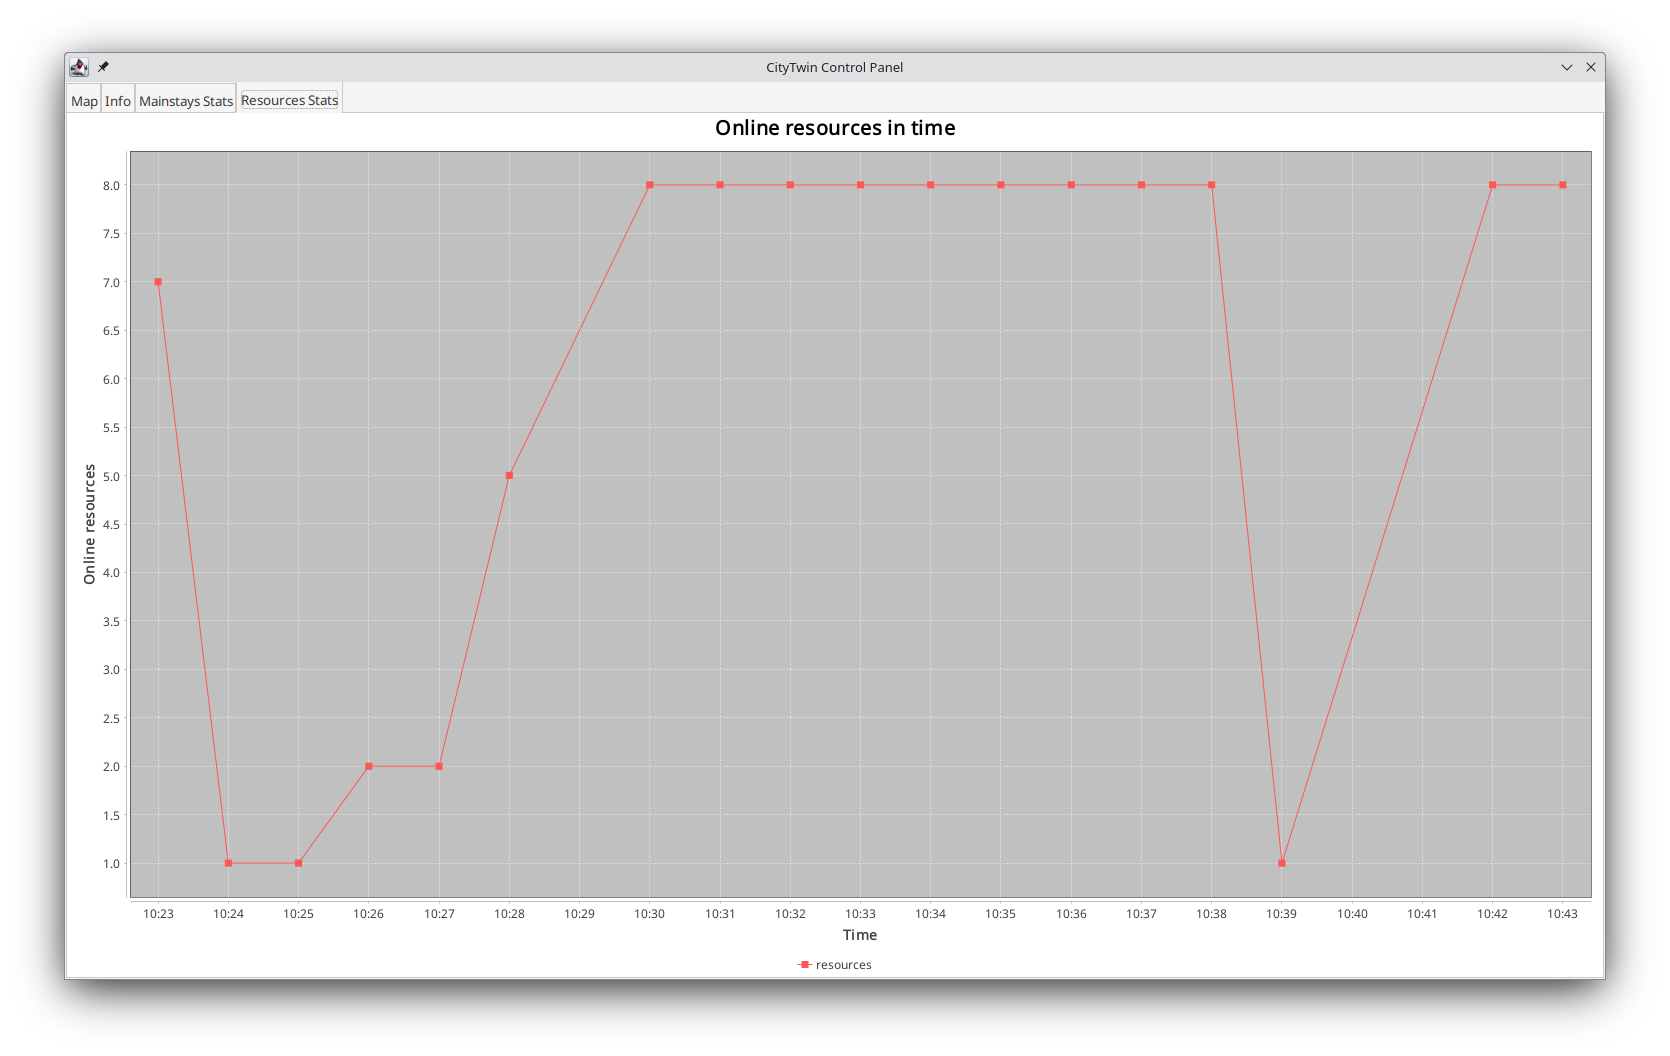
\includegraphics[width=\textwidth]{../assets/images/control-panel-resources-stats.png}
    \label{fig:control-panel-resources-stats}
\end{figure}

\subsection{Implementazione dei moduli Monitor}
In questa sezione verrà illustrata l'implementazione delle parti più significative dei moduli di monitoraggio dell'aria, delle piogge acide, dell'inquinamento acustico e delle alluvioni.

\subsubsection{Sensori}
Tutti e quattro i moduli Monitor implementano ognuno un proprio sensore, rappresentato da un attore specifico, che simula il comportamento di un sensore reale. I sensori dei quattro moduli seguono una struttura simile nell'implementazione, basata sull'utilizzo di attori e su un timer per la generazione periodica dei dati. Ciò che cambia da un sensore all'altro è il tipo di dato che viene generato e inviato al sistema.
Nel seguente listato viene mostrata l'implementazione di \textit{Flood Sensor Actor,
    Noise Sensor Actor, Air Sensor Actor} e \textit{Acid Rain Sensor Actor}, senza andare nel dettaglio dei dati generati.

\begin{lstlisting}[language=Scala]
object SensorActor:
  def apply(sensor: Sensor): Behavior[SensorActorCommand] =
    Behaviors.setup { ctx =>
      val resourceActor = ctx.spawnAnonymous(ResourceActor())
      Behaviors.withTimers { timers =>
        timers.startTimerAtFixedRate(Tick, TickInterval)
        Behaviors.receiveMessage {
          case Tick =>
            // Generate data
            val data = generateMeasurementData()
            val resource = Resource(
              Some(sensor.name),
              Some(sensor.position),
              Some(data),
              Set(ResourceType.Sense)
            )
            // Send generated data to ResourceActor
            resourceActor ! ResourceChanged(resource)
            Behaviors.same
        }
      }
    }
\end{lstlisting}

\paragraph{Generazione dei dati}
Come i dati vengono generati è illustrato di seguito:
\begin{itemize}
    \item \textbf{Air Sensor Actor:} Questo attore è stato progettato per simulare l'utilizzo di un sensore fisico reale che possa comunicare solo attraverso un protocollo di rete. Per questo motivo, il sensore non genera direttamente i dati, ma li ottiene interagendo con una funzione su Azure che simula il comportamento del sensore. L'\textit{Air Sensor Actor} richiede i dati alla funzione attraverso una richiesta HTTP GET e la funzione risponde con i dati in formato JSON. Un esempio di risposta è la seguente stringa: \textit{\{"pm10":46.29966, "pm25":33.35241, "nox":76.84502\}}.
    \item \textbf{Acid Rain Sensor Actor:} Questo attore genera i dati in modo casuale. I dati generati sono valori di pH compresi tra 0 e 14. Un esempio di valore generato è la seguente stringa in formato JSON: \textit{\{"ph":7.0\}}.
    \item \textbf{Noise Sensor Actor:} Questo attore genera il valore di decibel in modo casuale, con un range da 40 a 100 decibel (dB), e una descrizione relativa al livello di rumore. Un esempio di dato generato è la seguente stringa in formato JSON: \textit{\{"value (dB)":65, "description":"Moderate noise"\}}.
    \item \textbf{Flood Sensor Actor:} Questo attore genera il valore di livello dell'acqua in modo casuale, con un range da 0 a 20. Un esempio di dato generato è la seguente stringa: \textit{16}.
\end{itemize}

\subsubsection{River Monitor Actor}
Il \textit{River Monitor Actor} fa parte del modulo \textit{River Monitor}. Dovendo questo attore comunicare più dati e con la necessità che questi dati venissero poi facilmente utilizzati dalla \textit{View}, si è deciso di serializzare in formato JSON un'intera \textit{Case Class} contenente tutti i dati necessari, mostrata nel seguente listato:
\begin{lstlisting}[language=Scala]
case class RiverMonitorResourceState(
    riverMonitorState: String,
    threshold: Float,
    monitoredSensors: Option[Map[String, Map[String, String]]]
)
\end{lstlisting}
Per la serializzazione e relativa deserializzazione di questa \textit{Case Class} si è utilizzata la libreria \textit{upickle}\cite{upickle}. Questa libreria permette di serializzare e deserializzare strutture dati in formato JSON in modo semplice e veloce.

\newpage


%----------------------------------------------------------------------------------------
%	TESTING E PERFORMANCE
%----------------------------------------------------------------------------------------

\section{Testing e performance}

\subsection{Testing dei Moduli Sviluppati in Scala 3}

Per testare i moduli sviluppati in Scala 3 si è scelto di utilizzare il framework di testing ScalaTest\cite{scalatest} in combinazione con il TestKit fornito da Akka.

ScalaTest è un framework di testing per il linguaggio di programmazione Scala. È progettato per semplificare il processo di scrittura e esecuzione dei test nelle applicazioni Scala, fornendo una varietà di stili di testing e utilità per rendere più facile il testing delle applicazioni.

Per testare efficacemente le applicazioni Akka, viene utilizzato il "TestKit di Akka", che è un modulo appositamente progettato per il testing delle interazioni tra attori e per la simulazione dell'ambiente di esecuzione concorrente.

Il seguente listato mostra un esempio di specifica di test per il \textit{Resource Actor} del modulo \textit{Core}. Grazie al TestKit di Akka, è possibile simulare l'invio di messaggi in modo asincrono e verificare che il comportamento dell'attore sia conforme alle specifiche.

\lstinputlisting[language=Scala]{../assets/listings/AsyncTestingResourceSpec.scala}

\subsection{Testing del Servizio di Persistenza}

Postman\cite{postman} è un'applicazione che offre un'ampia gamma di strumenti per semplificare il processo di sviluppo, test e documentazione delle API. Le API sono punti di accesso che consentono a diverse applicazioni di comunicare tra loro, scambiando dati e funzionalità. Postman è ampiamente utilizzato dai team di sviluppo di software per testare, convalidare e interagire con le API in diversi scenari.

Il servizio di persistenza espone delle API web, le quali sono state testate utilizzando il software Postman (Figura: \ref{fig:postman}).

\begin{figure}[H]
    \caption{Testing delle API web del servizio di persistenza utilizzando Postman.}
    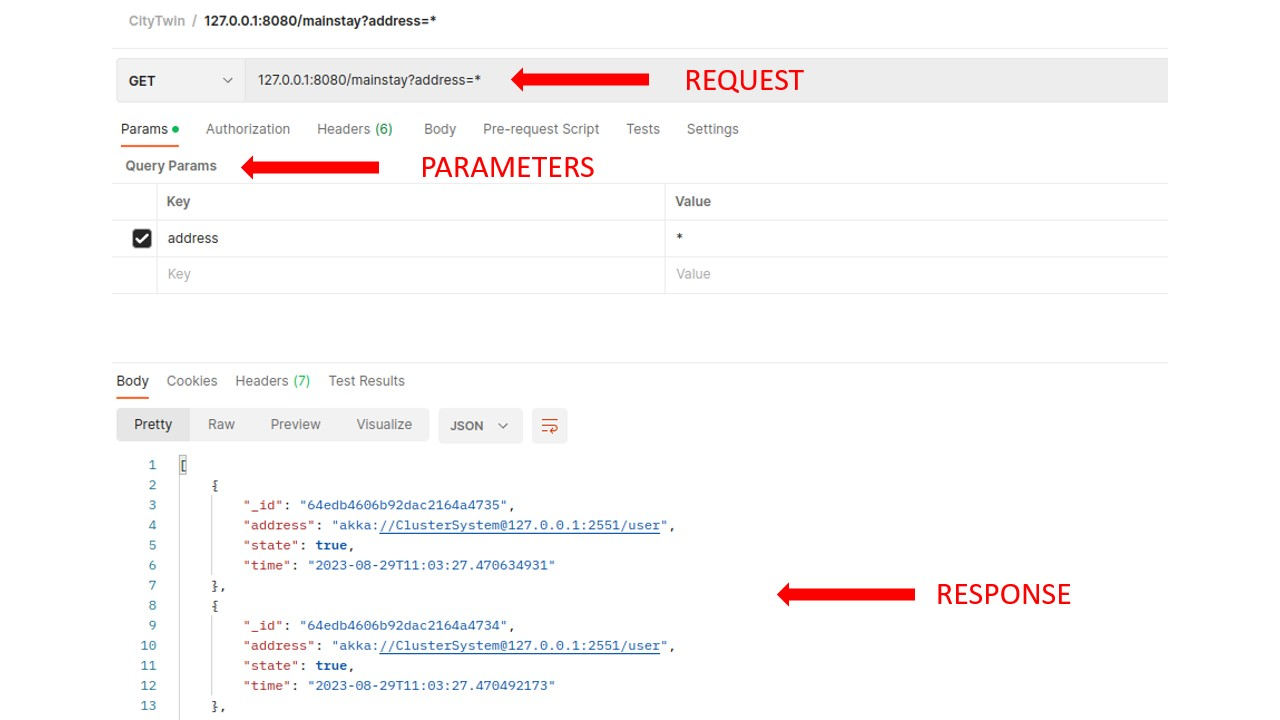
\includegraphics[width=\textwidth]{../assets/images/postman.jpg}
    \label{fig:postman}
\end{figure}

\subsection{Performance del Sistema Distribuito}

Per l'analisi delle performance del sistema distribuito si è scelto di considerare i tempi dello scambio dei messaggi tra uno dei nodi \textit{Resource} e il suo \textit{Mainstay} di riferimento. I risultati dell'analisi sono riportati in Tabella \ref{tab:analysis-specs}.

L'esecuzione è avvenuta in locale, su una macchina con le caratteristiche descritte in Tabella \ref{tab:machine-specs}.

\begin{figure}[H]
    \caption{Specifiche della macchina su cui è stata eseguita l'analisi.}
    \begin{center}
        \begin{tabular}{ | l | l | }
            \hline
            \textbf{OS}                   & NixOS 23.05       \\
            \hline
            \textbf{Linux kernel version} & 6.1.47            \\
            \hline
            \textbf{CPU}                  & AMD Ryzen 7 5700U \\
            \hline
            \textbf{Cores}                & 8                 \\
            \hline
            \textbf{Threads}              & 16                \\
            \hline
            \textbf{Base clock}           & 1.8GHz            \\
            \hline
            \textbf{Max boost clock}      & 4.3GHz            \\
            \hline
            \textbf{L2 cache}             & 4MB               \\
            \hline
            \textbf{L3 cache}             & 8MB               \\
            \hline
            \textbf{Memory}               & 15325MiB          \\
            \hline
        \end{tabular}
    \end{center}
    \label{tab:machine-specs}
\end{figure}

\begin{figure}[H]
    \caption{Risultati dell'analisi effettuata.}
    \begin{center}
        \begin{tabular}{ | l | l | }
            \hline
            \textbf{Numero di nodi \textit{Mainstay}} & 3       \\
            \hline
            \textbf{Numero di nodi \textit{Resource}} & 31      \\
            \hline
            \textbf{Numero di richieste effettuate}   & 101     \\
            \hline
            \textbf{Numero di risposte ottenute}      & 101     \\
            \hline
            \textbf{Tempo di risposta massimo}        & 3.228 s \\
            \hline
            \textbf{Tempo di risposta minimo}         & 0.002 s \\
            \hline
            \textbf{Tempo di risposta medio}          & 0.183 s \\
            \hline
        \end{tabular}
    \end{center}
    \label{tab:analysis-specs}
\end{figure}

%----------------------------------------------------------------------------------------
%	ANALISI DI DEPLOYMENT SU LARGA SCALA
%----------------------------------------------------------------------------------------

\section{Analisi di deployment su larga scala}

La presente sezione si concentra sull'analisi di deployment su larga scala di un sistema, considerando l'evoluzione del progetto da un contesto isolato a uno di dimensioni significative. L'obiettivo principale è valutare come garantire l'adeguata resilienza, disponibilità e scalabilità del sistema in tale scenario.

Il deployment su larga scala richiede una progettazione oculata e una solida implementazione. L'adozione di servizi cloud, l'architettura a microservizi e le best practice di sicurezza, unitamente a un monitoraggio costante, contribuiscono a garantire la resilienza, la disponibilità e la scalabilità del sistema. L'analisi e l'adeguamento delle risorse in termini di costo sono altresì rilevanti per un'implementazione di successo.

\subsection{Architettura a Microservizi}

Nel passaggio a una scala maggiore, l'adozione di un'architettura a microservizi emerge come una soluzione pragmatica. Questo approccio suddivide il sistema in componenti modulari indipendenti, semplificando la gestione e il deployment. Ogni microservizio può essere scalato separatamente in base alle esigenze di carico, migliorando l'efficienza e la manutenibilità complessiva.

\subsection{Infrastruttura Cloud}

L'utilizzo di una piattaforma cloud costituisce un aspetto chiave per garantire la flessibilità e la scalabilità necessarie. I servizi cloud, come AWS\cite{amazonaws}, Azure e GCP\cite{gcp}, offrono meccanismi automatici di scalabilità delle risorse in risposta al carico di lavoro. Questo non solo migliora la resilienza, ma permette anche una gestione efficiente delle risorse.

\subsection{Bilanciamento del Carico}

L'impiego di bilanciatori di carico risulta essenziale per distribuire uniformemente il traffico tra diverse istanze dei servizi. Questa pratica evita sovraccarichi e previene il single point of failure, garantendo la disponibilità continua del sistema anche in caso di aumento del traffico.

\subsection{Autoscaling}

L'implementazione di un sistema di autoscaling consente di adeguare dinamicamente il numero di istanze dei servizi in base alla domanda. Ciò si traduce in prestazioni ottimali durante i picchi di utilizzo e nell'uso efficiente delle risorse durante i periodi di minor carico, garantendo un'esperienza utente coerente.

\subsection{Tecnologie di Containerizzazione e Orchestrazione}

L'adozione di tecnologie di contenitori, come Docker, e sistemi di orchestrazione, come Kubernetes\cite{kubernetes}, agevola la distribuzione e la gestione dei servizi. La containerizzazione assicura l'isolamento delle applicazioni, mentre l'orchestrazione semplifica il deployment, il monitoraggio e la scalabilità.

\subsection{Backup e Ripristino}

Pianificare strategie di backup regolari e procedure di ripristino è fondamentale per assicurare la continuità operativa. In caso di guasti o perdita di dati, queste misure garantiscono l'integrità dei dati e riducono i tempi di inattività.

\subsection{Sicurezza}

Nel contesto di un deployment su larga scala, la sicurezza riveste un ruolo cruciale e richiede una considerazione approfondita.

Con un maggior numero di utenti e componenti, la gestione delle credenziali diventa complessa. L'uso di pratiche di autenticazione forte, come l'autenticazione a due fattori, e la centralizzazione delle credenziali attraverso strumenti di gestione delle identità contribuiscono a mitigare il rischio di accessi non autorizzati.

La sicurezza dei dati è fondamentale. L'adozione di crittografia dei dati in transito e a riposo previene l'accesso non autorizzato ai dati sensibili. Inoltre, è importante definire politiche di accesso rigorose e autorizzazioni granulari per limitare l'accesso solo alle parti necessarie del sistema.

Con l'aumento del traffico, il rischio di attacchi distribuiti di negazione del servizio (DDoS) aumenta. L'adozione di soluzioni di mitigazione DDoS e la configurazione dei bilanciatori di carico per filtrare il traffico dannoso contribuiscono a mantenere la disponibilità del sistema.

Eseguire test di penetrazione regolari può rivelare potenziali vulnerabilità che potrebbero essere sfruttate dagli attaccanti. Questi test simulano attacchi reali per identificare punti deboli nel sistema.

\newpage


%----------------------------------------------------------------------------------------
%	PIANO DI LAVORO
%----------------------------------------------------------------------------------------

\section{Piano di lavoro}

Per lo sviluppo del progetto è stato adottato un processo ispirato alle tecniche agili proposte da Scrum.
La prima attività intrapresa è stata quella di analizzare i requisiti del sistema. Lo sviluppo delle funzionalità si è articolato secondo unità di tempo, chiamate Sprint, che scandivano il ritmo con il quale venivano effettuate riunioni e confronti tra gli sviluppatori. Al termine di ogni sprint settimanale, il team si riuniva per effettuare una retrospettiva su quanto svolto, per definire ciò che restava da sviluppare ed eventuali difficoltà incontrate. Durante ogni sprint, per organizzare il lavoro da svolgere, è stato prodotto uno sprint backlog: un artefatto che tiene traccia delle funzionalità da sviluppare. Per quanto riguarda la definizione dei task è stata utilizzata la funzionalità "issue boards" di GitLab\cite{GitLab}, in questo modo è stato possibile tener traccia dello stato di avanzamento del progetto.

Di seguito viene riportato il process backlog effettuato durante lo sviluppo del progetto.

\begin{itemize}
    \item Sprint 1
          \begin{itemize}
              \item Obiettivi
                    \begin{itemize}
                        \item Impostare il progetto SBT @ Barzi
                        \item Aggiungere CI per automatizzare i test @ Vissani
                        \item Aggiungere la configurazione di Akka Cluster @ Vissani
                        \item Definire l'architettura del Core e iniziare l'implementazione @ Vissani, Barzi
                        \item Definire le impostazioni di logging @ Vissani
                        \item Definire lo scopo e avviare l'implementazione del modulo River Monitor @ Barzi
                    \end{itemize}
              \item Revisione
                    \begin{itemize}
                        \item Alcuni comportamenti del Core devono essere corretti
                        \item Deve essere deciso come le risorse interagiscono con i Mainstay
                        \item I progetti delle risorse concrete devono essere definiti
                    \end{itemize}
          \end{itemize}
\end{itemize}

\begin{itemize}
    \item Sprint 2
          \begin{itemize}
              \item Obiettivi
                    \begin{itemize}
                        \item Trovare un modo per inviare le HashMap nei messaggi @ Vissani
                        \item Definire il comportamento di ResourceActor @ Vissani
                        \item Rendere ResourceActor consapevole dei Mainstay online @ Vissani
                        \item Avviare l'implementazione del Control Panel @ Vissani
                        \item Definire i moduli delle risorse concrete @ Barzi
                        \item Continuare l'implementazione di River Monitor integrandolo con ResourceActor @ Barzi
                    \end{itemize}
              \item Revisione
                    \begin{itemize}
                        \item Alcuni comportamenti del Core devono essere risolti
                        \item L'implementazione del Control Panel non è completa
                        \item Bisogna trovare un modo semplice per avviare l'intero sistema distribuito
                    \end{itemize}
          \end{itemize}
\end{itemize}

\begin{itemize}
    \item Sprint 3
          \begin{itemize}
              \item Obiettivi
                    \begin{itemize}
                        \item Stabilizzare le API del Core @ Vissani
                        \item Dockerizzare le applicazioni @ Barzi
                        \item Continuare l'implementazione di River Monitor @ Barzi
                        \item Migliorare il Control Panel @ Vissani
                        \item Avviare l'implementazione del servizio di persistenza @ Vissani
                    \end{itemize}
              \item Revisione
                    \begin{itemize}
                        \item Non è stato possibile Dockerizzare le applicazioni a causa di Swing
                        \item Il comportamento del servizio di persistenza deve essere testato
                        \item Le interazioni con il servizio di persistenza devono essere implementate
                    \end{itemize}
          \end{itemize}
\end{itemize}

\begin{itemize}
    \item Sprint 4
          \begin{itemize}
              \item Obiettivi
                    \begin{itemize}
                        \item Implementare l'interazione tra Core e servizio di persistenza @ Vissani
                        \item Implementare l'interazione tra Control Panel e servizio di persistenza @ Vissani
                        \item Avviare l'implementazione di Air Quality Monitor @ Barzi
                        \item Avviare l'implementazione di Acid Rain Monitor @ Barzi
                        \item Avviare l'implementazione di Noise Pollution Monitor @ Barzi
                    \end{itemize}
              \item Revisione
                    \begin{itemize}
                        \item La sincronizzazione tra i Mainstay deve essere migliorata
                        \item L'implementazione dei moduli delle risorse deve essere completata
                        \item Le scritture non necessarie sul servizio di persistenza devono essere ridotte
                    \end{itemize}
          \end{itemize}
\end{itemize}

\begin{itemize}
    \item Sprint 5
          \begin{itemize}
              \item Obiettivi
                    \begin{itemize}
                        \item Migliorare la sincronizzazione tra i Mainstay @ Vissani
                        \item Aggiungere la possibilità di scegliere la mappa della città @ Vissani
                        \item Aggiungere la documentazione @ Vissani, Barzi
                    \end{itemize}
          \end{itemize}
\end{itemize}

\newpage


%----------------------------------------------------------------------------------------
%	CONCLUSIONI
%----------------------------------------------------------------------------------------

\section{Conclusioni}
In conclusione possiamo evidenziare come il progetto abbia raggiunto gli obiettivi prefissati, ovvero la realizzazione di un sistema distribuito per il monitoraggio di una Smart City. Il sistema è stato sviluppato in maniera modulare, in modo da poter essere facilmente esteso e mantenuto. Inoltre, il sistema è stato progettato per essere scalabile e resiliente, in modo da poter essere utilizzato in un contesto reale.

\subsection{Sviluppi futuri}
Tra i vari miglioramenti a cui abbiamo pensato, i più significativi sono:
\begin{itemize}
    \item Utilizzo di una mappa geografica reale (simile a \textit{Google Maps}): Integrare una mappa geografica reale all'interno del sistema, consentendo di posizionare le risorse virtuali in base alle coordinate reali delle smart city. Questo migliorerebbe la precisione della modellazione e consentirebbe una rappresentazione più accurata dell'ambiente urbano.
    \item Sviluppo delle interfacce grafiche con applicazioni web in modo da renderle accessibili da dispositivi di vario genere (computer, smartphone, tablet, ecc.).;
    \item Possibilità per le risorse di tipo \textit{Act} di accedere allo storico dei dati rendendo trasparente il servizio di persistenza;
    \item Sostituzione dei sensori virtualizzati con sensori reali, in modo da poter effettuare un deployment su larga scala in un contesto reale.
    \item Implementazione di un sistema di autenticazione e autorizzazione per garantire la sicurezza del sistema.
    \item Implementazione di un sistema di notifiche per avvisare gli utenti in caso di eventi critici.
    \item Espansione delle funzionalità di analisi con l'ausilio di sistemi \textit{Big Data}: Introduzione di capacità di analisi avanzate per estrarre insight più profondi dai dati raccolti, ad esempio, analisi predittive per prevedere eventi futuri o rilevare anomalie in tempo reale.
    \item Implementazione di AI e Machine Learning: Integrazione di algoritmi di intelligenza artificiale e machine learning per l'automazione delle decisioni basate sui dati e per migliorare l'efficienza operativa delle smart city.
\end{itemize}

\newpage

%----------------------------------------------------------------------------------------
%	RIFERIMENTI BIBLIOGRAFICI
%----------------------------------------------------------------------------------------
\addcontentsline{toc}{section}{Riferimenti bibliografici}
\bibliographystyle{plain}
\bibliography{bibliography}

%----------------------------------------------------------------------------------------

\end{document}